\date{}
\title{}
\date{}
\usepackage{pgfplots}
\pgfplotsset{compat=1.16}
\begin{document}
\begin{frame}
    \titlepage
\end{frame}

\begin{frame}{last time}
    \begin{itemize}
    \item using asymmetric encryption
    \item digital signatures
        \begin{itemize}
        \item sign with private key; verify with public key
        \end{itemize}
    \item replay attacks
    \item reflection attacks/mistaken identity
    \item nonces, other context
    \item logic errors evading cryptography
    \item cryptographic hashes; random numbers
    \end{itemize}
\end{frame}

\section{random numbers, briefly}
\begin{frame}{random numbers}
    \begin{itemize}
    \item want keys, etc. to be unguessable and evenly distributed
    \vspace{.5cm}
    \item solution: random numbers
    \item but: many random number functions are not cryptographically secure!
        \begin{itemize}
        \item example NOT SECURE: \sout{C \texttt{rand()}; Python's \texttt{random.random}}
        \item better: Python's \texttt{secrets}, \texttt{os.urandom}; Linux \texttt{getrandom()}, \texttt{/dev/urandom}
        \end{itemize}
    \vspace{.5cm}
    \item extra effort to ensure \myemph{not guessable}
    \item need to incorporate ``entropy'' from unpredictable sources
        \begin{itemize}
        \item deliberately unstable circuit; exact timing of input/output; etc.
        \end{itemize}
    \end{itemize}
\end{frame}


\section{key agreement}
\begin{frame}{just asymmetric?}
    \begin{itemize}
    \item given public-key encryption + digital signatures\ldots
    \item why bother with the symmetric stuff?
    \vspace{.5cm}
    \item symmetric stuff much faster
    \item symmetric stuff much better at supporting larger messages
    \end{itemize}
\end{frame}

\begin{frame}{key agreement}
    \begin{itemize}
    \item problem: A has B's public encryption key \\
        wants to choose shared secret 
    \vspace{.5cm}
    \item some ideas:
        \begin{itemize}
        \item A chooses a key, sends it encrypted to B
        \item A sends a public key encrypted B, B chooses a key and sends it back
        \end{itemize}
    \item<2-> alternate model:
        \begin{itemize}
        \item both sides generate random values
        \item derive public-key like ``key shares'' from values
        \item use math to combine ``key shares''
        \item kinda like A + B both sending each other public encryption keys
        \end{itemize}
    \end{itemize}
\end{frame}

\begin{frame}{Diffie-Hellman key agreement (2)}
\begin{itemize}
\item A and B want to agree on shared secret
\vspace{.5cm}
\item A chooses random value Y
\item A sends public value derived from Y (``key share'')
\item B chooses random value Z
\item B sends public value derived from Z (``key share'')
\item A combines Y with public value from B to get number
\item B combines Z with public value from B to get number
    \begin{itemize}
    \item and b/c of math chosen, both get same number
    \end{itemize}
\end{itemize}
\end{frame}

\begin{frame}{Diffie-Hellman key agreement (1)}
    \begin{itemize}
    \item math requirement:
        \begin{itemize}
        \item some $f$, so $f(f(X, Y), Z) = f(f(X, Z), Y)$
        \item (that's hard to invert, etc.)
        \end{itemize}
    choose X in advance and:
    \end{itemize}
\begin{tabular}{l|l}
A randomly chooses $Y$ & B randomly chooses $Z$ \\
A sends $f(X, Y)$ to B & B sends $f(X, Z)$ to A \\
A computes $f(f(X, Z), Y)$ & B computes $f(f(X, Y), Z)$ \\
\end{tabular}
\end{frame}



\section{putting it together: TLS}

\subsection{handshake}
\usetikzlibrary{arrows.meta,shapes.callouts,positioning}

\begin{frame}{typical TLS handshake}
\begin{tikzpicture}
    \tikzset{
        >=Latex,
        comp box/.style={draw, thick, align=center, minimum width=1.5cm,minimum height=6.25cm},
        explain box/.style={draw=red,very thick, align=left},
        msg/.style={font=\small},
        cmd/.style={font=\small},
    }
        \node[comp box] (client) at (-6.5, 0) {client};
        \node[draw,cloud,line width=1pt,minimum width=4cm,minimum height=2cm,aspect=3,opacity=0.25] (network) at (0,0) {~~};
        \node[comp box] (server) at (6.5, 0) {server};
        \draw[very thick,->] ([yshift=-.5cm]client.north east) -- ([yshift=-.5cm]server.north west) 
            node[midway,below,msg] (client key share) {ClientHello,KeyShare};
        \draw[very thick,<-] ([yshift=-1.5cm]client.north east) -- ([yshift=-1.5cm]server.north west) 
            node[midway,below,msg] (server key share) {ServerHello,KeyShare};
        \draw[very thick,<-] ([yshift=-2.5cm]client.north east) -- ([yshift=-2.5cm]server.north west) 
            node[midway,below,msg] (certificate) {Certificate,CertificateVerify};
        \draw[very thick,<-] ([yshift=-3.5cm]client.north east) -- ([yshift=-3.5cm]server.north west) 
            node[midway,below,msg] (finished1) {Finished};
        \draw[very thick,->] ([yshift=-4.5cm]client.north east) -- ([yshift=-4.5cm]server.north west) 
            node[midway,below,msg] (finished2) {Finished};
    \begin{visibleenv}<2>
        \node[my callout2=client key share,anchor=north] at ([yshift=-1cm]client key share) {
            KeyShare = key parts for key exchange
        };
    \end{visibleenv}
    \begin{visibleenv}<3>
        \node[my callout2=certificate,anchor=north,align=left] at ([yshift=-1cm]certificate) {
            Certificate = certificate (``foo.com's public key is X'' + CA signature) \\
            \myemph<3>{CertificateVerify = Sign(foo.com's private key, server's key share)}
        };
    \end{visibleenv}
    \begin{visibleenv}<4-5>
        \node[my callout2=finished1,anchor=north,align=left] at ([yshift=-1cm]finished1) {
            MAC(\myemph<4>{key made from key shares}, Hash(everything so far))
        };
    \end{visibleenv}
    \begin{visibleenv}<6>
        \node[my callout2=finished2,anchor=north,align=left] at ([yshift=-1cm]finished2) {
            MAC(\myemph<4>{key made from key shares}, Hash(everything so far))
        };
    \end{visibleenv}
\end{tikzpicture}
\end{frame}


\subsection{after handshake}
\begin{frame}{TLS: after handshake}
    \begin{itemize}
    \item use key shares results to get \textbf{several} keys
        \begin{itemize}
        \item take hash(something + shared secret) to derive each key
        \end{itemize}
    \item separate keys for each direction (server $\rightarrow$ client and vice-versa)
    \item often separate keys for encryption and MAC
    \vspace{.5cm}
    \item later messages use encryption + MAC + nonces
    \end{itemize}
\end{frame}


\subsection{TLS properties}
\begin{frame}{things modern TLS usually does}
    \begin{itemize}
        \item (not all these properties provided by all TLS versions and modes)
    \vspace{.5cm}
    \item confidentiality/authenticity 
        \begin{itemize}
        \item server = one ID'd by certificate
        \item client = same throughout whole connection
        \end{itemize}
    \item forward secrecy
        \begin{itemize}
        \item can't decrypt old conversations (data for KeyShares is temporary)
        \end{itemize}
    \item fast
        \begin{itemize}
        \item most communication done with more efficient symmetric ciphers
        \item 1 set of messages back and forth to setup connection
        \end{itemize}
    \end{itemize}
\end{frame}




\makeatletter
\newenvironment<>{btHighlight}[1][]
{\begin{onlyenv}#2\begingroup\tikzset{bt@Highlight@par/.style={#1}}\begin{lrbox}{\@tempboxa}}
{\end{lrbox}\bt@HL@box[bt@Highlight@par]{\@tempboxa}\endgroup\end{onlyenv}}

\newcommand<>\btHL[1][]{%
  \only#2{\begin{btHighlight}[#1]\bgroup\aftergroup\bt@HL@endenv}%
}
\def\bt@HL@endenv{%
  \end{btHighlight}%   
  \egroup %
}
\tikzset{
    btHLbox/.style={
        fill=red!30,outer sep=0pt,inner xsep=1pt, inner ysep=0pt, rounded corners=3pt
    },
}
\newcommand{\bt@HL@box}[2][]{%
  \tikz[#1]{%
    \pgfpathrectangle{\pgfpoint{1pt}{0pt}}{\pgfpoint{\wd #2}{\ht #2}}%
    \pgfusepath{use as bounding box}%
    \node[text width={},draw=none,anchor=base west, btHLbox, minimum height=\ht\strutbox+1pt,#1]{\raisebox{1pt}{\strut}\strut\usebox{#2}};
  }%
}

\lst@CCPutMacro
    \lst@ProcessOther {"2A}{%
      \lst@ttfamily 
         {\raisebox{2pt}{*}}% used with ttfamily
         {\raisebox{2pt}{*}}}% used with other fonts
    \@empty\z@\@empty

\lstdefinelanguage
   [x8664gas]{Assembler}     % add a "x64" dialect of Assembler
   [x86masm]{Assembler} % based on the "x86masm" dialect
   % with these extra keywords:
   {morekeywords={CDQE,CQO,CMPSQ,CMPXCHG16B,JRCXZ,LODSQ,MOVSXD,%
                  POPFQ,PUSHFQ,SCASQ,STOSQ,IRETQ,RDTSCP,SWAPGS,.TEXT,.STRING,.ASCIZ,%
                  BEQ,LW,SW,LB,SB,ADDIU,J,BEQZ,BNEZ,BNE,%
                  MOVUPD,MULPD,MOVSD,MULSD,%
                  SHLADD,MOV,CMP.LT,TBIT.NZ,BR.RET.SPTK.MANY,%
                  ADDQ,POPQ,PUSHQ,RRMOVQ,MRMOVQ,RMMOVQ,IRMOVQ,%
                  <-,LL,SC,ADDI,ADDL,VMOVDQA,ADDQ,CMPL,JB,JBE,MOVL,CLTQ,
                  MOVW,PUSHW,MOV,ADD,SUB,INT,PUSH,MOV,ADD,REP,MOVSB,%
                  TESTQ,CMPQ,MOVL,MOVQ,ADDQ,JMPQ,XORQ,%
                  LEAQ,LEAL,LEA,RETQ,RET,POPL,POPW,PUSHL,PUSHW,%
                  LEAW,%
                  SUBQ,SYSCALL,.ASCII,CALLQ,MOVSLQ,JMP,ANDQ,SHRQ,MOVB,INCQ,TESTL,XORL,%
                  SHRL,LEAL,SARL,SUBL,IMULL,IMULQ,MOVDQU,PADDD,XORL,%
                  MOVZBL,MOVZB,SHRB,SRAL,SHRL,ANDL,%
                  CMOVNS,SRAL,SRAQ,MOVZBW,MOVZBQ,%
                  PADDW,PADDQ,MODUPS,MOVAPD,%
                  MOVL,RET,.GLOBL,%
                  },
    deletekeywords={eax,ebx,sp,si,cx,di,ds,cs,es,fs,dx,ax,bx,al,esi,ebp,ecx,rip,eip,edx,edi,rdi,esp},
    morecomment=[l]{\#},
    morecomment=[l]{\/\/},
    morecomment=[s]{/*}{*/},
    sensitive=false,
    keepspaces=true} % et

\lstalias[]{myasm}[x8664gas]{Assembler}

\lstdefinelanguage{JavaScript}{
  keywords={typeof, new, true, false, catch, function, return, null, catch, switch, var, if, in, while, do, else, case, break},
  ndkeywords={class, export, boolean, throw, implements, import, this},
  sensitive=false,
  comment=[l]{//},
  morecomment=[s]{/*}{*/},
  morestring=[b]',
  morestring=[b]"
}

\newcommand{\keywordstyle}{\sourcecodeprolight\bfseries\color{blue!30!black}}
\newcommand{\stringstyle}{\color{blue!20!black}\ttfamily}

\lstset{
    language=C,
    basicstyle=\sourcecodepro\EmptyMapping,
    escapechar=`,
    keywordstyle=\keywordstyle\EmptyMapping,
    identifierstyle=\sourcecodepro\EmptyMapping,
    numberstyle=\small\color{black!70},
    commentstyle=\color{red!60!black}\ttfamily\itshape,
    stringstyle=\color{blue!20!black}\ttfamily,
    ndkeywordstyle=\bfseries\color{blue!30!black},
    upquote=true,
}



\lstdefinestyle{medium}{
    basicstyle=\sourcecodepro\EmptyMapping\fontsize{12}{13}\selectfont,
    keywordstyle=\sourcecodepro\EmptyMapping\fontsize{12}{13}\selectfont\keywordstyle,
}

\lstdefinestyle{small}{
    basicstyle=\sourcecodepro\EmptyMapping\small,
    keywordstyle=\sourcecodepro\EmptyMapping\small\keywordstyle,
}

\lstdefinestyle{smaller}{
    basicstyle=\sourcecodepro\EmptyMapping\fontsize{11}{12}\selectfont,
    keywordstyle=\sourcecodepro\EmptyMapping\fontsize{11}{12}\selectfont\keywordstyle,
}


\lstdefinestyle{script}{
    basicstyle=\sourcecodepro\EmptyMapping\scriptsize,
    keywordstyle=\sourcecodepro\EmptyMapping\scriptsize\bfseries,
}



\usetikzlibrary{circuits.logic.mux}
\makeatletter
\pgfdeclareshape{myregister}%
{
    \inheritsavedanchors[from=rectangle]
    \inheritanchorborder[from=rectangle]
    \inheritanchor[from=rectangle]{center}
    \inheritanchor[from=rectangle]{north}
    \inheritanchor[from=rectangle]{south}
    \inheritanchor[from=rectangle]{west}
    \inheritanchor[from=rectangle]{east}
    \inheritanchor[from=rectangle]{north east}
    \inheritanchor[from=rectangle]{north west}
    \inheritanchor[from=rectangle]{south east}
    \inheritanchor[from=rectangle]{south west}
    \inheritbackgroundpath[from=rectangle]
    \saveddimen{\halfbaselength}{%
         \pgf@x=0.5\wd\pgfnodeparttextbox
         % get xsep
         \pgfmathsetlength\pgf@xc{\pgfkeysvalueof{/pgf/inner xsep}}%
         \advance\pgf@x by \pgf@xc%
         % get \ht of textbox, add to baselength 
         \advance\pgf@x by \wd\pgfnodeparttextbox
         % get minimum width
         \pgfmathsetlength\pgf@xb{\pgfkeysvalueof{/pgf/minimum width}}%
         \divide\pgf@xb by 2
         \ifdim\pgf@x<\pgf@xb%
             % yes, too small. Enlarge...
             \pgf@x=\pgf@xb%
         \fi%
     }
    \backgroundpath{
        \pgfpathrectanglecorners{\southwest}{\northeast}
        \southwest \pgf@xa=\pgf@x \pgf@ya=\pgf@y 
        \pgf@yb=\pgf@ya
        \northeast \pgf@xb=\pgf@x %\pgf@yb=\pgf@y
        \pgf@xc = \pgf@xa
        \advance\pgf@xc by \halfbaselength
        \pgf@yc=\pgf@ya
        \advance\pgf@yc by \halfbaselength
        \pgfpathmoveto{\pgfpoint{\pgf@xa}{\pgf@ya}}
        \pgfpathlineto{\pgfpoint{\pgf@xc}{\pgf@yc}}
        \pgfpathlineto{\pgfpoint{\pgf@xb}{\pgf@yb}}
        \pgfpathclose
    }
}
\makeatother

\usetikzlibrary{arrows.meta}
\usetikzlibrary{fit}

\providecommand{\cpuset}{
\tikzset{
    box/.style={draw,very thick,align=center},
    cache/.style={box,fill=yellow!20,minimum width=2cm,minimum height=1.5cm},
    regfile/.style={box,fill=blue!20,minimum height=3cm,align=center},
    alu/.style={box,fill=violet!20,minimum height=1.5cm,minimum width=2cm},
    pc/.style={box,myregister,label={center:PC},minimum height=2cm,minimum width=.75cm,fill=yellow!30},
    connect/.style={draw,ultra thick,-Latex},
}
}
\providecommand{\cpucomponent}{
\node[pc] (pc) {};
\node[cache,anchor=west] (icache) at ([xshift=1cm]pc.east) {I\$};
\node[anchor=north,box,font=\small] (ilen) at ([yshift=-.25cm]icache.south) {+ instr\\len};
\node[regfile,anchor=north west] (regfile) at ([yshift=.5cm,xshift=1cm]icache.east) {register\\file};
\node[alu,anchor=west] (math) at ([xshift=1cm]regfile.east |- pc.east) {math};
\node[cache,anchor=west] (dcache) at ([xshift=1cm,yshift=-1cm]math.east) {D\$};
\node[anchor=north,font=\small] at ([yshift=-.1cm]regfile.north) {read};
\node[anchor=south east,font=\small] at ([yshift=.25cm]regfile.south east) {write};
}
\providecommand{\cpuconnect}{
\draw[connect] (pc) -- (icache);
\draw[connect] (pc.east) -- ++(0.5cm,0cm) |- (ilen.west);
\draw[connect] (ilen.east) -- ++(0.25cm,0cm) |- ([yshift=-1.5cm,xshift=-.5cm]pc.south west) |- (pc.west);
\coordinate (pre pc) at ([xshift=-.5cm,yshift=-1.5cm]pc.west);

\draw[connect] ([yshift=-.25cm]icache.north east) -- ([yshift=-.25cm]math.north west)
    coordinate[midway] (decode middle top) coordinate (math in top);
\draw[connect] ([yshift=-1cm]icache.north east) |- ([yshift=-1cm]icache.north east -| regfile.west) coordinate (regfile read in);

\draw[connect] ([yshift=-1cm]icache.north east -| regfile.east) coordinate (regfile read out) -- ([yshift=-1cm]math.north west) coordinate (reg to math);
\draw[connect] ([yshift=.5cm]math.south east) coordinate (math out 2) -- ([yshift=.5cm]math.south east -| dcache.west) coordinate (math to cache);
\draw[connect] ([yshift=-.5cm]math.north east) coordinate (math out 1) -- ([yshift=-.5cm,xshift=.75cm]math.north east -| dcache.east)
    |- ([xshift=.75cm,yshift=-.5cm]dcache.south east) -- ([yshift=-.5cm]dcache.south -| regfile.east);
\coordinate (memory top) at ([yshift=1cm]dcache.north);
\draw[connect] (dcache.east) -- ++(0.35cm,0cm) |- ([yshift=-.25cm]dcache.south -| regfile.east)
    coordinate (regfile write in);
\coordinate (regfile write in opposite) at (regfile write in -| regfile.west);
}

\providecommand{\stagestyles}{
\tikzset{
    stage/.style={draw,line width=1mm,opacity=0.7,fill opacity=0.2},
    fetch/.style={draw=yellow,fill=yellow},
    decode/.style={draw=orange,fill=orange},
    execute/.style={draw=green,fill=green},
    memory/.style={draw=blue,fill=blue},
    writeback/.style={draw=violet,fill=violet},
    fd reg/.style={draw=yellow!50!orange,fill=yellow!30!orange!30},
    de reg/.style={draw=orange!50!green,fill=orange!30!green!30},
    em reg/.style={draw=green!50!blue,fill=green!30!blue!30},
    mw reg/.style={draw=blue!50!violet,fill=blue!30!violet!30},
}
}
\providecommand{\stageboxes}{
    \node[stage,fetch,fit=(icache) (ilen),label={north:fetch}] (fetch) {};
    \node[stage,decode,fit=(regfile read in) (regfile read out) (decode middle top),label={north:decode}] (decode) {};
    \node[stage,execute,fit=(math in top) (math),label={north:execute}] (execute) {};
    \node[stage,memory,fit=(dcache) (memory top),label={north:memory}] (memory) {};
    \node[stage,writeback,fit=(regfile write in) (regfile write in opposite) (regfile.south),label={south:writeback}] (writeback) {};
}
\providecommand{\stageregs}{
    \node[draw,myregister,anchor=north,very thick,minimum width=0.1cm,minimum height=2cm,fd reg] (fd reg) at ([xshift=.25cm,yshift=0.25cm]fetch.north east) {};
    \node[draw,myregister,anchor=north,very thick,minimum width=0.1cm,minimum height=2cm,de reg] (de reg) at ([xshift=.25cm,yshift=0.25cm]decode.north east) {};
    \node[draw,myregister,anchor=north,very thick,minimum width=0.1cm,minimum height=3cm,em reg] (em reg) at ([xshift=.25cm,yshift=0.25cm]execute.north east) {};
    \node[draw,myregister,anchor=north,very thick,minimum width=0.1cm,minimum height=1cm,mw reg] (mw reg) at ([xshift=.5cm,yshift=0.25cm]writeback.north east) {};
}

\tikzset{
    matrix stages/.style={
        row 1 column 2/.append style={nodes={fill=yellow!20}},
        row 1 column 3/.append style={nodes={fill=orange!20}},
        row 1 column 4/.append style={nodes={fill=green!20}},
        row 1 column 5/.append style={nodes={fill=blue!20}},
        row 1 column 6/.append style={nodes={fill=violet!20}},
        nodes={text depth=0.2ex},
    },
    hiBox/.style={fill=red,opacity=0.2},
}


\section{review: single-cycle proccesor}

% FIXME: CPU design, example execution
\begin{frame}{simple CPU}
\begin{tikzpicture}
\cpuset
\cpucomponent
\cpuconnect
\end{tikzpicture}
\end{frame}

\begin{frame}{running instructions}
\begin{tikzpicture}
\cpuset
\cpucomponent
\cpuconnect
\node[draw,font=\tt\small,ultra thick,anchor=north west,align=left] (code) at ([yshift=-3cm]pc.south west) {
    0x100: \myemph<2>{addq \%r8, \%r9} \\
    0x108: \myemph<3>{movq 0x1234(\%r10), \%r11} 
};
\node[fill=blue!20,draw,font=\tt\small,ultra thick,anchor=north west,align=left] at ([xshift=.5cm,yshift=.5cm]code.north east) {
    \ldots \\
    \%r8: 0x800 \\
    \%r9: \alt<1>{0x900}{\myemph<2>{0x1100}} \\
    \%r10: 0x1000 \\
    \%r11: \alt<1-2>{0x1100}{\myemph<3>{M[0x2234]}} \\
    \ldots
};
\tikzset{
    hilite/.style={font=\small\tt,red,fill=white,fill opacity=0.8,inner sep=0.05mm,align=center},
};
\begin{visibleenv}<2>
\node[hilite] at ([yshift=.5cm]pc) {0x100};
\node[hilite] at (pre pc) {0x108};
\node[hilite,anchor=east,align=left] at (regfile read in) {8\\9};
\node[hilite,anchor=west,align=left] at (regfile read out) {0x800\\0x900};
\node[hilite,anchor=west,align=left] at (math out 1) {0x1100};
\end{visibleenv}
\begin{visibleenv}<3>
\node[hilite] at ([yshift=.5cm]pc) {0x108};
\node[hilite] at (pre pc) {0x110};
\node[hilite,anchor=east,align=left] at (regfile read in) {10};
\node[hilite,anchor=west,align=left] at (regfile read out) {0x1000};
\node[hilite,anchor=west,align=left] at (math out 2) {0x2234};
\node[hilite,anchor=west,align=left] at (regfile write in) {M[0x2234]};
\end{visibleenv}
\end{tikzpicture}
\end{frame}


\section{pipelining idea}

\subsection{laundry idea}
\usetikzlibrary{patterns}

\newcommand<>{\laundryLabels}[1]{%
\begin{visibleenv}#2
\begin{scope}[every node/.style={font=\small,text width=1.5cm,anchor=east,draw,rectangle,minimum height=1cm,
    inner sep=1pt,fill=white}]
    \node (washer) at (1, {#1-1}) {Washer};
    \node (dryer) at (1, {#1-2}) {Dryer};
    \node (table) at (1, {#1-3}) {Folding Table};
\end{scope}
\begin{scope}[every node/.style={font=\scriptsize,anchor=south,append after command={
    [very thick] ($(\tikzlastnode.south) + (0cm,0mm)$)edge($(\tikzlastnode.south) + (0cm,1mm)$)
}}]
    \node at (1,{#1-.5}) {11:00};
    \node at (4,{#1-.5}) {12:00};
    \node at (7,{#1-.5}) {13:00};
    \node at (10,{#1-.5}) {14:00};
\end{scope}
\end{visibleenv}
}
\tikzset{
    laundryNode/.style={draw,rectangle,anchor=west,minimum height=1cm,inner xsep=1pt,
                        font=\fontsize{12.5}{13}\selectfont},
    extra/.style={execute at begin node={},fill=green!50!black},
    extra2/.style={execute at begin node={},fill=violet!30!white},
    whites/.style={execute at begin node={\color{white}whites},fill=black!70},
    colors/.style={execute at begin node={\color{blue!70}colors},fill=red!10},
    sheets/.style={execute at begin node={\color{black}sheets},fill=blue!30!white},
    wasted/.style={laundryNode,pattern=north west lines,draw=none,pattern color=red},
    fade/.style={opacity=0.1},
    fadeWeak/.style={opacity=0.4},
}

\newcommand<>{\laundryLoadNoPipe}[6]{
\begin{visibleenv}#7
\node[minimum width=#3cm,laundryNode,#6] at ({#2+0}, {#1-1}) {};
\node[minimum width=#4cm,laundryNode,#6] at ({#2+#3}, {#1-2}) {};
\node[minimum width=#5cm,laundryNode,#6] at ({#2+#3+#4}, {#1-3}) {};
\end{visibleenv}
}

\newcommand<>{\laundryLoadStraight}[6]{
\begin{visibleenv}#7
\node[minimum width=#3cm,laundryNode,#6] at ({#2+0}, {#1}) {};
\node[minimum width=#4cm,laundryNode,#6] at ({#2+#3}, {#1}) {};
\node[minimum width=#5cm,laundryNode,#6] at ({#2+#3+#4}, {#1}) {};
\end{visibleenv}
}

\newcommand<>{\laundryLoadPipe}[6]{
\begin{visibleenv}#7
\node[minimum width=#3cm,laundryNode,#6] at ({#2+0}, {#1-1}) {};
\node[minimum width=#4cm,laundryNode,#6] at ({#2+max(#3,#4)}, {#1-2}) {};
\node[minimum width=#5cm,laundryNode,#6] at ({#2+2*max(#3,#4)}, {#1-3}) {};
\end{visibleenv}
}


\newcommand<>{\laundryLoadNoPipeDefault}[3]{
\laundryLoadNoPipe#4{#1}{#2}{1.5}{1.7}{1.3}{#3}
}
\newcommand<>{\laundryLoadPipeDefault}[3]{
\laundryLoadPipe#4{#1}{#2}{1.5}{1.7}{1.3}{#3}
}

\newcommand<>{\laundryLoadPipeLong}[3]{
\laundryLoadPipe#4{#1}{#2}{1.5}{2.5}{1.3}{#3}
}
\newcommand<>{\laundryLoadNoPipeLong}[3]{
\laundryLoadNoPipe#4{#1}{#2}{1.5}{2.5}{1.3}{#3}
}
\newcommand<>{\laundryLoadStraightLong}[3]{
\laundryLoadStraight#4{#1}{#2}{1.5}{2.5}{1.3}{#3}
}

\usetikzlibrary{positioning,calc,shapes.callouts}

\begin{frame}{Human pipeline: laundry}
\small
\begin{tikzpicture}
\laundryLabels{0}
\begin{visibleenv}<2-|handout:1>\laundryLabels{-4}\end{visibleenv}
\laundryLoadNoPipeDefault{0}{1}{whites}
\laundryLoadNoPipeDefault{0}{5.5}{colors}

\laundryLoadNoPipeDefault<2-|handout:1->{-4}{1}{whites}
\laundryLoadPipeDefault<2-|handout:1->{-4}{1+1.5}{colors}
\laundryLoadPipeDefault<2-|handout:1->{-4}{1+1.5+1.7}{sheets}
\end{tikzpicture}
\end{frame}

\begin{frame}{Waste (1)}
\begin{tikzpicture}
\laundryLabels{0}
\laundryLoadNoPipeDefault{0}{1}{whites}
\laundryLoadPipeDefault{0}{1+1.5}{colors}
\laundryLoadPipeDefault{0}{1+1.5+1.7}{sheets}
\node[minimum width=0.2cm,wasted] at ({1+1.5+1.5},-1) (waste1) {};
\node[minimum width=0.2cm,wasted] at ({1+1.5+1.7+1.5},-1) (waste2) {};
\begin{visibleenv}<2->
\node[my callout2=waste2.north,fill=red!30!white] at ([yshift=2cm]waste1.north) {wasted time!};
\node[my callout2=waste1.north,fill=red!30!white] at ([yshift=2cm]waste1.north) {wasted time!};
\end{visibleenv}
\end{tikzpicture}
\end{frame}

\begin{frame}{Waste (2)}
\begin{tikzpicture}
\laundryLabels{0}
\laundryLoadNoPipeLong{0}{1}{whites}
\laundryLoadPipeLong{0}{1+1.5}{colors}
\laundryLoadPipeLong{0}{1+1.5+2.5}{sheets}
\node[minimum width=1cm,wasted] at ({1+1.5+1.5},-1) (waste1) {};
\node[minimum width=1cm,wasted] at ({1+1.5+2.5+1.5},-1) (waste2) {};
\end{tikzpicture}
\end{frame}

\begin{frame}{Latency --- Time for One}
\begin{tikzpicture}
\laundryLabels{0}
\laundryLoadNoPipeLong{0}{1}{whites,fade}
\laundryLoadPipeLong{0}{1+1.5}{colors}
\laundryLoadPipeLong{0}{1+1.5+2.5}{sheets,fade}
\node[minimum width=1cm,wasted] at ({1+1.5+1.5},-1) (waste1) {};
\begin{visibleenv}<2->
\coordinate (colorsStart) at ({1+1.5},-3.5);
\coordinate (colorsEnd) at ({1+1.5+2.5+2.5+1.3},-3.5);
\draw[very thick,red] (colorsStart) -- ++(0,3);
\draw[very thick,red] (colorsEnd) -- ++(0,3);
\draw[very thick,red,Latex-Latex] ([yshift=-.1cm]colorsStart) -- ([yshift=-.1cm]colorsEnd)
    node[midway,below] {pipelined latency (2.1 h)};
\end{visibleenv}
\begin{visibleenv}<3->
\laundryLoadStraightLong{-5}{1+1.5}{colors}
\node[minimum width=1cm,wasted,anchor=east] at ([yshift=-1.5cm]colorsEnd) {};
\draw[very thick,blue,Latex-Latex] ([yshift=-2.2cm]colorsStart) -- ([yshift=-2.2cm,xshift=-1cm]colorsEnd)
    node[midway,below] {normal latency (1.8 h)};
\end{visibleenv}
\end{tikzpicture}
\end{frame}

\begin{frame}{Throughput --- Rate of Many}
\begin{tikzpicture}
\laundryLabels{0}
\begin{pgfonlayer}{bg}
\laundryLoadNoPipeLong{0}{1-1.5}{extra,fadeWeak}
\end{pgfonlayer}
\laundryLoadPipeLong{0}{1}{whites}
\laundryLoadPipeLong{0}{1+2.5}{colors}
\laundryLoadPipeLong{0}{1+2.5+2.5}{sheets}
\laundryLoadPipeLong{0}{1+2.5+2.5+2.5}{extra}
\laundryLoadPipeLong{0}{1+2.5+2.5+2.5+2.5}{extra2}
\coordinate (whitesEnd) at ({1+2.5+2.5+1.3},-3.5);
\coordinate (colorsEnd) at ({1+2.5+2.5+2.5+1.3},-3.5);
\draw[very thick,red] ([yshift=-1cm]whitesEnd) -- ++(0,2);
\draw[very thick,red] ([yshift=-1cm]colorsEnd) -- ++(0,2);
\draw[very thick,red,Latex-Latex] ([yshift=-1.1cm]whitesEnd) -- ([yshift=-1.1cm]colorsEnd)
    node[xshift=-1cm,midway,below,black] (timeBetweenE){time between finishes (0.83 h)};
\begin{visibleenv}<2->
    \node[below=.2cm of timeBetweenE] {
        $\frac{1 \text{ load}}{0.83 \text{h}} = \color{red}1.2 \text{ loads/h}$
    };
\end{visibleenv}
\begin{visibleenv}<3->
    \coordinate (colorsStart) at ({1+2.5},-3.5);
    \coordinate (sheetsStart) at ({1+2.5+2.5},-3.5);
    \draw[very thick,red] (colorsStart) -- ++(0,3);
    \draw[very thick,red] (sheetsStart) -- ++(0,3);
    \draw[very thick,red,Latex-Latex] ([yshift=-.1cm]colorsStart) -- ([yshift=-.1cm]sheetsStart)
        node[xshift=-1cm,midway,below,black] (timeBetweenS){time between starts (0.83 h)};
\end{visibleenv}
\end{tikzpicture}
\end{frame}



\subsection{applying to single-cycle processor}
\usetikzlibrary{fit,matrix}

\begin{frame}{adding stages (one way)}
\begin{tikzpicture}
\cpuset
\cpucomponent
\cpuconnect
\stagestyles
\begin{pgfonlayer}{fg}
    \stageboxes
\end{pgfonlayer}
\begin{visibleenv}<1>
\node[draw=red,line width=.5mm,anchor=north,align=left] at ([yshift=-1cm]regfile.south) {
    divide running instruction into steps \\
    one way: fetch / decode / execute / memory / writeback
};
\end{visibleenv}
\begin{pgfonlayer}{fg}
    \begin{visibleenv}<2->
    \stageregs
    \end{visibleenv}
\end{pgfonlayer}
\begin{visibleenv}<2>
\node[draw=red,line width=.5mm,anchor=north,align=left] at ([yshift=-1cm]regfile.south) {
    add `pipeline registers' to hold values from instruction
};
\end{visibleenv}
\end{tikzpicture}
\end{frame}

\newcommand{\fdemw}{ \& |[fetch]| F \& |[decode]| D \& |[execute]| E \& |[memory]| M \& |[writeback]| W}
\begin{frame}{running some instructions}
\begin{tikzpicture}
\cpuset
\cpucomponent
\cpuconnect
\stagestyles
\begin{pgfonlayer}{fg}
    \stageboxes
    \stageregs
    \begin{visibleenv}<2->
        \matrix[tight matrix no line,
                nodes={text width=.6cm,font=\tt,minimum height=.7cm,align=center,text opacity=1.0,fill opacity=0.5},
                column 1/.style={nodes={text width=9cm,align=left}},anchor=north west] (tbl) 
                    at ([xshift=-1cm,yshift=-2cm]pc.south){
        |[align=right]| \normalfont\textit{cycle \#} \hspace{.5cm}
                                            \& 0 \& 1 \& 2 \& 3 \& 4 \& 5 \& 6 \& 7 \& 8 \\
        0x100: add \%r8, \%r9    \fdemw \& ~ \& ~ \& ~ \& ~ \& ~ \& ~\\
        0x108: mov 0x1234(\%r10), \%r11  \& ~ \fdemw \& ~ \& ~\\
        0x110: xor \%r12, \%r13  \& ~ \& ~ \fdemw \& ~ \& ~\\
        };
    \end{visibleenv}
    \tikzset{
        hilite/.style={font=\fontsize{10}{11}\selectfont\tt,red,fill=white,fill opacity=0.8,inner sep=0.05mm,align=center},
    };
    \begin{visibleenv}<2>
        \node[inner sep=0mm,draw=red,ultra thick,fit=(tbl-1-2) (tbl-4-2)] {};
        \node[hilite] at ([yshift=.5cm]pc) {0x100\\(add)};
        \node[hilite] at (pre pc) {0x108};
    \end{visibleenv}
    \begin{visibleenv}<3>
        \node[inner sep=0mm,draw=red,ultra thick,fit=(tbl-1-3) (tbl-4-3)] {};
        \node[hilite,anchor=west,align=left] at ([xshift=-.25cm]regfile read in) {8 (for add)\\9 (for add)};
        \node[hilite] at ([yshift=.5cm]pc) {0x108\\(mov)};
        \node[hilite] at (pre pc) {0x110};
    \end{visibleenv}
    \begin{visibleenv}<4>
        \node[inner sep=0mm,draw=red,ultra thick,fit=(tbl-1-4) (tbl-4-4)] {};
        \node[hilite] at ([yshift=.5cm]pc) {0x110\\(xor)};
        \node[hilite,anchor=west,align=left] at ([xshift=-.25cm]regfile read in) {10 (for mov)};
        \node[hilite,anchor=west,align=left] at ([xshift=1cm]regfile read out) {0x800 (r8)\\0x900 (r9)};
    \end{visibleenv}
    \begin{visibleenv}<5>
        \node[inner sep=0mm,draw=red,ultra thick,fit=(tbl-1-5) (tbl-4-5)] {};
        \node[hilite,anchor=west,align=left] at ([xshift=-.25cm]regfile read in) {12 (for xor)\\13 (for xor)};
        \node[hilite,anchor=west,align=left] at ([xshift=1cm]regfile read out) {0x1234 \\ 0x1000 (r10)};
        \node[hilite,anchor=west,align=left] at ([xshift=1cm]math out 1) {0x1100 (sum)};
    \end{visibleenv}
    \begin{visibleenv}<6>
        \node[inner sep=0mm,draw=red,ultra thick,fit=(tbl-1-6) (tbl-4-6)] {};
        \node[hilite,anchor=east,align=left] at ([xshift=0cm]regfile write in) {0x1100 (sum)};
        \node[hilite,anchor=west,align=left] at ([xshift=1cm]regfile read out) {0x1200 (r12)\\0x1300 (r13)};
        \node[hilite,anchor=west,align=left] at ([xshift=1cm]math out 2) {0x2234 (mov addr)};
    \end{visibleenv}
\end{pgfonlayer}
\end{tikzpicture}
\end{frame}

\begin{frame}{why registers?}
    \begin{itemize}
    \item example: fetch/decode
    \item need to store current instruction somewhere \ldots while fetching next one
    \end{itemize}
\end{frame}



\subsection{exercise: throughput/latency}
\usetikzlibrary{fit,matrix}


\begin{frame}{exercise: throughput/latency (1)}
\begin{tikzpicture}
    \stagestyles
    \providecommand{\fdemw}{ \& |[fetch]| F \& |[decode]| D \& |[execute]| E \& |[memory]| M \& |[writeback]| W}
    \matrix[tight matrix no line,
            nodes={text width=.6cm,font=\tt,minimum height=.7cm,align=center,text opacity=1.0,fill opacity=0.5},
            column 1/.style={nodes={text width=9cm,align=left}},anchor=north west] (tbl) {
    |[align=right]| \normalfont\textit{cycle \#} \hspace{.5cm}
                                        \& 0 \& 1 \& 2 \& 3 \& 4 \& 5 \& 6 \& 7 \& 8 \\
    0x100: add \%r8, \%r9    \fdemw \& ~ \& ~ \& ~ \& ~ \& ~ \& ~\\
    0x108: mov 0x1234(\%r10), \%r11  \& ~ \fdemw \& ~ \& ~\\
    0x110: \ldots \& ~ \& ~ \& ~ \& \ldots \\
    };
\end{tikzpicture}
\begin{itemize}
\item support cycle time is 500 ps
\item exercise: latency of one instruction?
{\small\begin{tabular}{lllll}
A. 100 ps & B. 500 ps & C. 2000 ps & D. 2500 ps & E. something else \\
\end{tabular}}
\item<2-> exercise: throughput overall?
{\small\begin{tabular}{llll}
A. 1 instr/100 ps & B. 1 instr/500 ps & C. 1 instr/2000ps & D. 1 instr/2500 ps \\
 E. something else \\
\end{tabular}}
\end{itemize}
\end{frame}

\begin{frame}{exercise: throughput/latency (2)}
\begin{tikzpicture}
    \stagestyles
    \providecommand{\fdemw}{ \& |[fetch]| F \& |[decode]| D \& |[execute]| E \& |[memory]| M \& |[writeback]| W}
    \matrix[tight matrix no line,
            nodes={text width=1.2cm,font=\tt,minimum height=.7cm,align=center,text opacity=1.0,fill opacity=0.5},
            column 1/.style={nodes={text width=9cm,align=left}},anchor=north west] (tbl1) {
    |[align=right]| \normalfont\textit{cycle \#} \hspace{.5cm}
                                        \& 0 \& 1 \& 2 \& 3 \& 4 \& 5 \& 6 \& 7 \& 8 \\
    0x100: add \%r8, \%r9    \fdemw \& ~ \& ~ \& ~ \& ~ \& ~ \& ~\\
    0x108: mov 0x1234(\%r10), \%r11  \& ~ \fdemw \& ~ \& ~\\
    0x110: \ldots \& ~ \& ~ \& ~ \& \ldots \\
    };
    \providecommand{\ffdemw}{ \& |[fetch]| F1 \& |[fetch]| F2
                             \& |[decode]| D1 \& |[decode]| D2 
                             \& |[execute]| E1 \& |[execute]| E2
                              \& |[memory]| M1 \& |[memory]| M2
                               \& |[writeback]| W1 \& |[writeback]| W2}
    \matrix[tight matrix no line,anchor=north,
            nodes={text width=0.6cm,font=\tt,minimum height=.7cm,align=center,text opacity=1.0,fill opacity=0.5},
            column 1/.style={nodes={text width=9cm,align=left}},anchor=north west] (tbl2) at ([yshift=-0.2cm]tbl1.south west) {
    |[align=right]| \normalfont\textit{cycle \#} \hspace{.5cm}
                                        \& 0 \& 1 \& 2 \& 3 \& 4 \& 5 \& 6 \& 7 \& 8 \\
    0x100: add \%r8, \%r9    \ffdemw \& ~ \& ~ \& ~ \& ~ \& ~ \& ~\\
    0x108: mov 0x1234(\%r10), \%r11  \& ~ \ffdemw \& ~ \& ~\\
    0x110: \ldots \& ~ \& ~ \& ~ \& \ldots \\
    };
\end{tikzpicture}
\begin{itemize}
\item suppose we double number of pipeline stages (to 10) and
    decrease cycle time from 500 ps to 250 ps
\item exercise: new throughput?
{\small\begin{tabular}{llll}
A. 1 instr/100 ps & B. 1 instr/250 ps & C. 1 instr/1000ps & D. 1 instr/5000 ps \\
 E. something else \\
\end{tabular}}
\end{itemize}
\end{frame}


\subsubsection{slowest stage matters}
\usetikzlibrary{arrows.meta,shapes.misc,chains}
\usepgfplotslibrary{fillbetween}

\tikzset{
    hReg/.style={draw,myregister,minimum width=.4cm,minimum height=2cm,label={[font=\small,align=center]-90:#1}},
}

\begin{frame}<0>[label=deeperPipeline]{deeper pipeline}
\countStyles
\circuitStyles
\begin{tikzpicture}
    \renewcommand{\plusTwo}{+4}
    \renewcommand{\plusOne}{+2}
    \timesThreePipeStuff
    \begin{pgfonlayer}{fg}
        \begin{scope}[every node/.style={color=red!70!black,ultra thick}]
        \node[hRegSmall={$A$ ($t+3$)},fill=white] at ([yshift=-.2cm]alu1.center |- alu2.-130) {};
            \node[hReg={$2\times A$ \\ partial results},fill=white] (split1) at (alu1.center) {};
            \alt<5-6|handout:2>{
                \node[opacity=0.2,hReg={},fill=white] (ghostSplit2) at (alu2.center) {};
                \node[color=red,hReg={$3\times A$ \\ partial results},fill=white] (split2) at ([xshift=.25cm]alu2.center) {};
            }{
                \node[hReg={$3\times A$ \\ partial results},fill=white] (split2) at (alu2.center) {};
            }
        \end{scope}
    \end{pgfonlayer}
    \coordinate (timelineBase) at ($(aInput.south)+(0cm,-2.5cm)$);
    \foreach \basis/\ref in {OneReg/aInput,OneHalfReg/split1,TwoReg/twoTimesReg,TwoHalfReg/split2,ThreeReg/threeTimesReg} {
        \coordinate (before\basis) at ([xshift=-.25cm]\ref.west);
        \coordinate (after\basis) at ([xshift=.25cm]\ref.east);
    }

    \foreach \basis/\alu/\reg in {OneAdd/alu1/OneHalfReg,TwoAdd/alu2/TwoHalfReg} {
        \coordinate (beforeHalf\basis) at ([xshift=-1cm]\alu.west);
        \coordinate (afterHalf\basis) at (before\reg);
        \coordinate (before\basis) at (after\reg);
        \coordinate (after\basis) at ([xshift=1cm]\alu.east);
    }
    \coordinate (timelineBaseLow) at ($(aInput.south)+(0cm,-3.5cm)$);
    \begin{visibleenv}<2-|handout:1>
    \foreach \basis/\len in {OneReg/$10$ ps,HalfOneAdd/$25$ ps,OneAdd/$25$ ps,OneHalfReg/$10$ ps,TwoReg/$10$ ps,HalfTwoAdd/$25$ ps,TwoHalfReg/$10$ ps,TwoAdd/$25$ ps,ThreeReg/$10$ ps} {
        \begin{scope}[very thick,Latex-Latex]
            \draw (before\basis |- timelineBase) -- (after\basis |- timelineBase)
                node[midway,below,font=\scriptsize] (timeline-\basis) {\len};
        \end{scope}
    }
    \end{visibleenv}
    \begin{visibleenv}<3|handout:1>
        \begin{scope}[overlay]
       \node[anchor=west] at ([yshift=-1cm]beforeOneReg |- timelineBaseLow) {exercise: throughput now?};
        \end{scope}
    \end{visibleenv}
    \begin{visibleenv}<4|handout:2>
        \begin{scope}[overlay]
       \node[anchor=west,align=left] at ([yshift=-1cm]beforeOneReg |- timelineBaseLow) {exercise: throughput now? \\
        A. 1/(25 ps) \hspace{1cm} B. 1/(30 ps) \hspace{1cm} \\ C. 1/(35 ps) \hspace{1cm} D. something else};
        \end{scope}
    \end{visibleenv}
    \begin{visibleenv}<5|handout:2>
        \iftoggle{heldback}{}{
        \begin{scope}[overlay]
        \draw[very thick,red,Latex-Latex] (beforeOneReg |- timelineBaseLow) -- (afterHalfOneAdd |- timelineBaseLow)
            node[below right, xshift=-2.5cm]{throughput: $\frac{1}{35 \text{ ps}} \approx 28$ G ops/sec};
        \end{scope}
        }
    \end{visibleenv}
    \begin{visibleenv}<6-8|handout:3>
        \begin{scope}[overlay]
        \node[cross out,red,thick,draw] (crossOut1) at (timeline-HalfTwoAdd.center) {};
        \node[below=0cm of crossOut1,red,font=\small] {30 ps};
        \node[cross out,red,thick,draw] (crossOut2) at (timeline-TwoAdd.center) {};
        \node[below=0cm of crossOut2,red,font=\small] {20 ps};
        \end{scope}
    \end{visibleenv}
    \begin{visibleenv}<6|handout:3>
        \begin{scope}[overlay]
            \node[anchor=west] at ([yshift=-1cm]beforeOneReg |- timelineBaseLow) {exercise: throughput now? (didn't split second add evenly)};
        \end{scope}
    \end{visibleenv}
    \begin{visibleenv}<7|handout:4>
        \begin{scope}[overlay]
            \node[anchor=west,align=left] at ([yshift=-1cm]beforeOneReg |- timelineBaseLow) {exercise: throughput now? (didn't split second add evenly) \\
            A. 1/(25 ps) \hspace{1cm} B. 1/(30 ps) \hspace{1cm} \\
            C. 1/(35 ps) \hspace{1cm} D. 1/(40 ps) \hspace{1cm} E. something else};
        \end{scope}
    \end{visibleenv}
    \begin{visibleenv}<8|handout:5>
        \iftoggle{heldback}{}{
        \begin{scope}[overlay]
        \draw[very thick,red,Latex-Latex] (beforeTwoReg |- timelineBaseLow) -- (afterHalfTwoAdd |- timelineBaseLow)
            node[below right, xshift=-2.5cm]{throughput: $\frac{1}{40 \text{ ps}} \approx 25$ G ops/sec};
        \end{scope}
        }
    \end{visibleenv}
\end{tikzpicture}
\begin{visibleenv}<9->
    \vspace{0cm}
    \begin{itemize}
        \item Problem: \myemph<10|handout:3>{How much faster can we get?}
        \item Problem: \myemph<11|handout:4>{Can we even do this?}
    \end{itemize}
\end{visibleenv}
\end{frame}

\begin{frame}[fragile,label=diminishDelay]{diminishing returns: register delays}
\begin{tikzpicture}
    \tikzset{
        logic/.style 2 args={draw,rectangle,align=center,anchor=north west,minimum width=#1,on chain,join,
                      inner sep=4pt,outer sep=1pt,minimum height=0.75cm,
                      label={[font=\small]-90:#2},fill=blue!30,font=\scriptsize},
        myl/.style 2 args={label={[align=right]180:#2 ps\\per cycle}},
        myReg/.style={hReg={10 ps},minimum height=0.75cm,on chain,join},
        every join/.style={-Latex,very thick},
        my chain/.style={start chain,node distance=5mm},
    }
    \matrix {
    \begin{scope}[my chain]
        \node[logic={5cm}{100 ps},myl={1 stage}{110}] {logic (all)};
        \node[myReg] {};
    \end{scope} \\
    \begin{scope}[my chain]
        \node[logic={2.5cm}{50 ps},myl={2 stage}{60}] {logic (1/2)};
        \node[myReg] {};
        \node[logic={2.5cm}{50 ps}] {logic (2/2)};
        \node[myReg] {};
    \end{scope} \\
    \begin{scope}[my chain]
        \node[logic={1.5cm}{33 ps},myl={5 stage}{43}] {logic (1/3)};
        \node[myReg] {};
        \node[logic={1.5cm}{33 ps}] {logic (2/3)};
        \node[myReg] {};
        \node[logic={1.5cm}{33 ps}] {logic (3/3)};
        \node[myReg] {};
    \end{scope} \\
    \begin{scope}[my chain, node distance=20mm, every node/.style={inner sep=0pt}]
        \node[on chain] {\vdots};
        \node[on chain] {\vdots};
        \node[on chain] {\vdots};
        \node[on chain] {\vdots};
    \end{scope}
    \\
    \begin{scope}[my chain,node distance=7mm]
        \node[logic={0.1cm}{1 ps},myl={100 stage}{11}] {\strut};
        \node[myReg] {};
        \node[logic={0.1cm}{1 ps}] {\strut};
        \node[myReg] {};
        \node[logic={0.1cm}{1 ps}] {\strut};
        \node[myReg] {};
        \node[logic={0.1cm}{1 ps}] {\strut};
        \node[myReg] {};
        \node[on chain,join] {\ldots};
    \end{scope} \\
    };
\end{tikzpicture}
\end{frame}

% FIXME: graph
\begin{frame}[fragile,label=regDelayLat]{diminishing returns: register delays}
\begin{tikzpicture}
\begin{axis}[width=.95\textwidth,height=0.8\textheight,xlabel={number of stages},ylabel={time per completion (ps)},
    xmin=0.5,xmax=15.5,ymin=0,ymax=120]
    \addplot[domain=1:15,samples=15,only marks,blue] {100/x+10}
        coordinate[pos=0] (t0)
        coordinate[pos=1/14] (t1)
        coordinate[pos=13/14] (t13)
        coordinate[pos=14/14] (t14);
    \path[name path=ten] (0,10) -- (16, 10);
    \path[name path=zero] (0,0) -- (16, 0);
    \only<2->{
        \addplot+[pattern=north west lines,opacity=0.2] fill between[of=ten and zero];
        \node[anchor=center] at (8,5) { register delay };
    }
    \only<3->{
        \draw[red] (t0) -| (t1) node[near start, right] {1.83x speedup};
        \draw[red] (t13) -| (t14) node[near start, above, xshift=-1cm] {1.02x speedup};
    }
\end{axis}
\end{tikzpicture}
\end{frame}

\begin{frame}[fragile,label=regDelayThru]{diminishing returns: register delays}
\begin{tikzpicture}
\begin{axis}[width=.95\textwidth,height=0.8\textheight,xlabel={number of stages},ylabel={throughput (ops/ns)},
    xmin=0.5,xmax=15.5,ymin=0,ymax=105]
    \addplot[domain=1:15,samples=15,only marks,blue] {1000/(100/x+10)}
        coordinate[pos=0] (t0)
        coordinate[pos=1/14] (t1)
        coordinate[pos=13/14] (t13)
        coordinate[pos=14/14] (t14);
    \draw[red] (t0) -| (t1) node[midway, right] {1.83x throughput};
    \draw[red] (t13) -| (t14) node[near start, above, xshift=-1.5cm] {1.02x throughput};
    \only<2->{
        \draw[red,dashed,line width=1pt] (0,100) -- (16,100)
            node[midway,below] {max. rate of register updates};
    }
\end{axis}
\end{tikzpicture}
\end{frame}


\begin{frame}[fragile,label=diminishSplit]{diminishing returns: uneven split}
\begin{itemize}
    \item Can we split up some logic (e.g. adder) arbitrarily?
    \item Probably not...
\end{itemize}
\begin{tikzpicture}
    \tikzset{
        logic/.style 2 args={draw,rectangle,align=center,anchor=north west,minimum width=#1,on chain,
                      inner sep=4pt,outer sep=1pt,minimum height=0.75cm,
                      label={[font=\small]-90:#2},fill=blue!30,font=\scriptsize},
        myl/.style 2 args={label={[align=right]180:#2 ps\\per cycle}},
        myReg/.style={hReg={10 ps},minimum height=0.75cm,on chain},
        every join/.style={-Latex,very thick},
        my chain/.style={start chain,node distance=0mm},
    }
    \matrix {
    \begin{scope}[my chain]
        \node[logic={5cm}{100 ps},myl={1 stage}{110}] {logic (all)};
        \node[myReg] {};
    \end{scope} \\
    \begin{scope}[my chain]
        \node[logic={3cm}{\myemph<2>{60 ps}},myl={2 stage}{70}] {logic (1/2)};
        \node[myReg] {};
        \node[logic={2.5cm}{\myemph<2>{45 ps}}] {logic (2/2)};
        \node[myReg] {};
    \end{scope} \\
    \begin{scope}[my chain]
        \node[logic={2cm}{\myemph<3>{40 ps}},myl={3 stage}{50}] {logic\\(1/3)};
        \node[myReg] {};
        \node[logic={2cm}{\myemph<3>{40 ps}}] {logic\\(2/3)};
        \node[myReg] {};
        \node[logic={1.5cm}{\myemph<3>{30 ps}}] {logic\\(3/3)};
        \node[myReg] {};
    \end{scope} \\
    \begin{scope}[my chain, node distance=20mm, every node/.style={inner sep=0pt}]
        \node[on chain] {\vdots};
        \node[on chain] {\vdots};
        \node[on chain] {\vdots};
        \node[on chain] {\vdots};
    \end{scope}
    \\
    };
\end{tikzpicture}
\end{frame}



\section{challenge: hazards}

\subsection{data hazards intro}

\subsubsection{example execution: wrong result, stalling resolution}
\usetikzlibrary{matrix,fit}
\begin{frame}[fragile,label=addqDataHazard]{a data hazard}
\begin{tikzpicture}[overlay,remember picture]
\node[anchor=north east] at ([xshift=-.5cm,yshift=-1cm]current page.north east)
    {\resizebox{!}{0.16\textwidth}{\usebox{\pipeCpuBox}}};
\end{tikzpicture}
\lstset{
    style=small,
    moredelim=**[is][\btHL<2|handout:0>]{@2@}{@},
    moredelim=**[is][\btHL<3|handout:0>]{@3@}{@},
    moredelim=**[is][\btHL<4|handout:0>]{@4@}{@},
    moredelim=**[is][\btHL<5|handout:0>]{@5@}{@},
}
\begin{lstlisting}
// initially %r8 = 800,
//           %r9 = 900, etc.
addq %r8, %r9   // R8 + R9 -> R9
addq %r9, %r8   // R9 + R8 -> R9
addq ...
addq ...        
\end{lstlisting}
\begin{tikzpicture}
\matrix[tight matrix,nodes={text width=1cm,font=\scriptsize\tt},
        column 8/.append style={nodes={text width=1.2cm}},
        column 10/.append style={nodes={text width=1.2cm}},
        row 1/.append style={nodes={font=\scriptsize}},
        row 2/.append style={nodes={font=\scriptsize}},
        ] (tbl) {
 \& |[fill=yellow!10!white,align=center]| fetch \& rA \& rB \& R[rA] \& R[rB] \& rB \& sum \& rB \& sum \& rB \\
cycle \& PC \& rA \& rB \& R[rB] \& R[rB] \& rB \& sum \& rB \& sum \& rB \\
0 \& 0x0 \\
1 \& 0x2 \& 8  \& 9    \\ 
2 \&     \& 9  \& 8   \& 800  \& 900 \& 9 \\
3 \&     \&    \&     \& 900 \&  800 \& 8  \& 1700 \& 9 \\
4 \&     \&    \&     \&      \&      \&    \& 1700 \& 8  \& 1700 \& 9 \\
5 \&     \&    \&     \&      \&       \&    \&      \&   \& 1700 \& 8 \\
};
\begin{scope}[every node/.style={draw,inner sep=0pt},
              every label/.style={font=\scriptsize,draw=none}]
    \node[fit=(tbl-1-3) (tbl-1-4),fill=yellow!50!orange!10!white,label={center:fetch/decode}] {};
    \node[fit=(tbl-1-5) (tbl-1-7),fill=orange!50!green!10!white,label={center:decode/execute}] {};
    \node[fit=(tbl-1-8) (tbl-1-9),fill=green!50!blue!10!white,label={center:execute/memory}] {};
    \node[fit=(tbl-1-10) (tbl-1-11),fill=blue!50!violet!10!white,label={center:memory/writeback}] {};
\end{scope}

\begin{visibleenv}<2->
\node[red,draw,thick,label={[red]-90:should be 1700},fit=(tbl-6-5)] {};
\end{visibleenv}
\end{tikzpicture}
\end{frame}

\begin{frame}[fragile,label=DataHazardTime]{data hazard}
\begin{lstlisting}
addq %r8, %r9  // (1)
addq %r9, %r8  // (2)
\end{lstlisting}
\begin{tikzpicture}
\matrix[tight matrix,
    nodes={execute at begin node={\strut}},
    column 1/.append style={nodes={text width=1.4cm}},
    column 2/.append style={nodes={text width=6cm}},
    column 3/.append style={nodes={text width=4cm}},
    ] {
step\# \& pipeline implementation \& ISA specification\\
1      \& read r8, r9 for (1) \& read r8, r9 for (1) \\
2      \& read r9, r8 for (2) \& write r9 for (1) \\
3      \& write r9 for (1) \& read r9, r8 for (2) \\
4      \& write r8 for (2) \& write r8 ror (2) \\
};
\end{tikzpicture}
\begin{itemize}
\item pipeline reads \myemph{older value}\ldots
\item instead of value ISA says was just written
\end{itemize}
\end{frame}

\begin{frame}[fragile,label=dataHazardNoop]{data hazard compiler solution}
\begin{lstlisting}[style=small]
addq %r8, %r9
nop
nop
addq %r9, %r8
\end{lstlisting}
\begin{itemize}
\item one solution: \myemph{change the ISA}
    \begin{itemize}
    \item all \lstinline|addq|s take effect \myemph{three instructions later} \\
        (assuming can read register value while it is being written back)
    \end{itemize}
\item make it \myemph{compiler's  job}
\item problem: recompile everytime processor changes?
\end{itemize}
\end{frame}

\begin{frame}[fragile,label=dataHazardStall]{data hazard hardware solution}
\begin{lstlisting}[style=small]
addq %r8, %r9
// hardware inserts: nop
// hardware inserts: nop
addq %r9, %r8
\end{lstlisting}
\begin{itemize}
    \item how about hardware add nops?
    \item called \myemph{stalling}
    \item extra logic:
        \begin{itemize}
        \item sometimes don't change PC
        \item sometimes put do-nothing values in pipeline registers
        \end{itemize}
\end{itemize}
% FIXME: picture of MUX in front of PC, in front of fetch/decode
\end{frame}
\begin{frame}{stalling/nop pipeline diagram (1)}
\begin{tikzpicture}
    \stagestyles
    \providecommand{\fdemw}{ \& |[fetch]| F \& |[decode]| D \& |[execute]| E \& |[memory]| M \& |[writeback]| W}
        \matrix[tight matrix no line,
                nodes={text width=.6cm,font=\tt,minimum height=.7cm,align=center,text opacity=1.0,fill opacity=0.5},
                column 1/.style={nodes={text width=9cm,align=left}},anchor=north west] (tbl) {
        |[align=right]| \normalfont\textit{cycle \#} \hspace{.5cm}
                                            \& 0 \& 1 \& 2 \& 3 \& 4 \& 5 \& 6 \& 7 \& 8 \\
        add \%r8, \%r9    \fdemw \& ~ \& ~ \& ~ \& ~ \& ~ \& ~\\
        (nop) \& ~ \fdemw \& ~ \& ~\\
        (nop) \& ~ \& ~ \fdemw \& ~ \& ~\\
        addq \%r9, \%r8  \& ~ \& ~ \& ~ \fdemw \& ~ \& ~\\
        };
    \begin{visibleenv}<2>
        \node[draw=red,line width=1mm,inner sep=0mm,fit=(tbl-2-6)] {};
        \node[draw=red,line width=1mm,inner sep=0mm,fit=(tbl-5-6)] {};
        \draw[red,line width=1mm,dotted,->] (tbl-2-6) -- (tbl-5-6);
        \node[anchor=north,align=left] at (tbl.south) {assumption: \\
                if writing register value \\
                register file will return that value  for reads \\
                ~ \\
                not actually way register file worked in single-cycle CPU \\
                (e.g. can read old \%r9 while writing new \%r9)
            };
    \end{visibleenv}
\end{tikzpicture}
\end{frame}

\begin{frame}{stalling/nop pipeline diagram (2)}
\begin{tikzpicture}
    \stagestyles
    \providecommand{\fdemw}{ \& |[fetch]| F \& |[decode]| D \& |[execute]| E \& |[memory]| M \& |[writeback]| W}
        \matrix[tight matrix no line,
                nodes={text width=.6cm,font=\tt,minimum height=.7cm,align=center,text opacity=1.0,fill opacity=0.5},
                column 1/.style={nodes={text width=9cm,align=left}},anchor=north west] (tbl) {
        |[align=right]| \normalfont\textit{cycle \#} \hspace{.5cm}
                                            \& 0 \& 1 \& 2 \& 3 \& 4 \& 5 \& 6 \& 7 \& 8 \\
        add \%r8, \%r9    \fdemw \& ~ \& ~ \& ~ \& ~ \& ~ \& ~\\
        (nop) \& ~ \fdemw \& ~ \& ~\\
        (nop) \& ~ \& ~ \fdemw \& ~ \& ~\\
        |[fill=red!20]| (nop) \& ~ \& ~ \& ~  \fdemw \& ~ \& ~\\
        addq \%r9, \%r8  \& ~ \& ~ \& ~ \& ~\& ~ \fdemw \& ~ \& ~\\
        };
    \begin{visibleenv}<2>
        \node[draw=red,line width=1mm,inner sep=0mm,fit=(tbl-2-6)] {};
        \node[draw=red,line width=1mm,inner sep=0mm,fit=(tbl-6-7)] {};
        \draw[red,line width=1mm,dotted,->] (tbl-2-6) -- (tbl-6-7);
        \node[red,anchor=north] at (tbl.south) {
            if we didn't modify the register file, we'd need an extra cycle
            };
    \end{visibleenv}
\end{tikzpicture}
\end{frame}


\subsection{control hazards}
\usetikzlibrary{fit,matrix}

\begin{frame}[fragile,label=ControlFlowExample]{control hazard}
\begin{lstlisting}
cmpq %r8, %r9
je   0xFFFF
addq %r10, %r11
\end{lstlisting}
\begin{tikzpicture}
\matrix[tight matrix,nodes={text width=1cm,font=\scriptsize\tt},
        column 9/.append style={nodes={text width=1.8cm}},
        column 5/.append style={nodes={text width=0.8cm}},
        column 6/.append style={nodes={text width=2.2cm}},
        column 8/.append style={nodes={text width=0.8cm}},
        row 1/.append style={nodes={font=\scriptsize}},
        row 2/.append style={nodes={font=\scriptsize}},
        ] (tbl) {
 \& |[fill=yellow!10!white,align=center]| fetch \& rA \& rB  \& R[rA] \& R[rB] \& result \& \ldots \& \ldots \&\ldots  \\
cycle \& PC \& rA \& rB \& R[rA] \& R[rB] \& result \& \ldots \& \ldots \& \ldots \\
0 \& 0x0  \\
1 \& 0x2 \& 8  \& 9   \\ 
2 \& ??? \& --- \& --- \& 800  \& 900 \\
2 \& ??? \& --- \& --- \& --- \& --- \& less than \& ~ \& ~ \& ~ \\
};
\begin{scope}[every node/.style={draw,inner sep=0pt},
              every label/.style={font=\scriptsize,draw=none}]
    \node[fit=(tbl-1-3) (tbl-1-4),fill=yellow!50!orange!10!white,label={center:fetch$\rightarrow$decode}] {};
    \node[fit=(tbl-1-5) (tbl-1-6),fill=orange!50!green!10!white,label={center:decode$\rightarrow$execute}] {};
    \node[fit=(tbl-1-7) (tbl-1-8),fill=green!50!blue!10!white,label={center:execute$\rightarrow$writeback}] {};
    \node[fit=(tbl-1-8) (tbl-1-9),fill=blue!50!violet!10!white,label={center:execute$\rightarrow$writeback}] {};
\end{scope}
\begin{visibleenv}<2->
    \node[line width=2pt,draw,red,fit=(tbl-5-2),
          label={-45:{\tt 0xFFFF} if R[8] = R[9]; {\tt 0x12} otherwise}] {};
\end{visibleenv}
\end{tikzpicture}
\end{frame}

%\begin{frame}[fragile,label=ControlFlowExampleStall]{control hazard: stall}
%\begin{lstlisting}
%cmpq %r8, %r9
%// insert two nops
%je   0xFFFF
%addq %r10, %r11
%\end{lstlisting}
%\begin{tikzpicture}
%\matrix[tight matrix,nodes={text width=1cm,font=\scriptsize\tt},
%        column 9/.append style={nodes={text width=1.8cm}},
%        column 5/.append style={nodes={text width=0.8cm}},
%        column 8/.append style={nodes={text width=0.8cm}},
%        row 1/.append style={nodes={font=\scriptsize}},
%        row 2/.append style={nodes={font=\scriptsize}},
%        ] (tbl) {
% \& |[fill=yellow!10!white,align=center]| fetch \& rA \& rB  \& R[srcA] \& R[srcB] \& dstE \& next R[dstE] \& dstE \\
%cycle \& PC \& rA \& rB \& R[rA] \& R[rB] \& rB \& result \& rB \& result \& rB \\
%0 \& 0x0   \\
%1 \& 0x2*  \& 8  \& 9   \\ 
%2 \& 0x2*  \& 0xF  \& 0xF   \& 800  \& 900 \& 9 \\
%3 \& 0x2   \& 0xF  \& 0xF   \& --- \&  --- \& 0xF  \& 1700 \& 9 \\
%4 \& 0x10  \& 0xF  \& 0xF   \& --- \&  --- \& 0xF  \& ---  \& 0xF \\
%5 \&       \& 10  \& 11   \& --- \&  --- \& 0xF  \& ---  \& 0xF \\
%6 \&       \&     \&   \& 1000 \&  1100 \& 11 \& ---  \& 0xF \\
%};
%\begin{scope}[every node/.style={draw,inner sep=0pt},
%              every label/.style={font=\scriptsize,draw=none}]
%    \node[fit=(tbl-1-4) (tbl-1-5),fill=yellow!50!orange!10!white,label={center:fetch$\rightarrow$decode}] {};
%    \node[fit=(tbl-1-6) (tbl-1-8),fill=orange!50!green!10!white,label={center:decode$\rightarrow$execute}] {};
%    \node[fit=(tbl-1-9) (tbl-1-10),fill=green!50!blue!10!white,label={center:execute$\rightarrow$writeback}] {};
%\end{scope}
%\foreach \x/\base in {all:2/4,all:2/5,all:3/6} {
%    \begin{pgfonlayer}{bg}
%    \begin{visibleenv}<\x>
%        \pgfmathtruncatemacro{\fetchR}{\base}
%        \pgfmathtruncatemacro{\decodeR}{\base+1}
%        \pgfmathtruncatemacro{\executeR}{\base+2}
%        \pgfmathtruncatemacro{\writebackR}{\base+3}
%        \foreach \nd in {tbl-\decodeR-4,tbl-\decodeR-5,
%                         tbl-\executeR-6,tbl-\executeR-7,tbl-\executeR-8,
%                         tbl-\writebackR-9,tbl-\writebackR-10} {
%            \node[fit=(\nd),inner sep=0pt,fill=green,opacity=0.3] {};
%         }
%    \end{visibleenv}
%    \end{pgfonlayer}
%}
%\begin{visibleenv}<all:2>
%\node [fit=(tbl-4-2) (tbl-5-2), red, line width=2pt, draw, rounded corners,
%    label={[draw,fill=white,inner sep=1pt,line width=2pt]45:wait for two cycles for addq to update SF/ZF}] {};
%\end{visibleenv}
%\begin{visibleenv}<all:3>
%\node [fit=(tbl-6-2), red, line width=2pt, draw, rounded corners,
%    label={[draw,fill=white,inner sep=1pt,line width=2pt]45:execute je instruction (use SF/ZF)}] {};
%\end{visibleenv}
%\end{tikzpicture}
%\end{frame}
%
 % FIXME: correct

\subsubsection{idea: branch prediction}
\usetikzlibrary{matrix, fit}
\begin{frame}[fragile,label=jCCStall]{jXX: stalling?}
\begin{tikzpicture}
    \stagestyles
    \providecommand{\fdemw}{ \& |[fetch]| F \& |[decode]| D \& |[execute]| E \& |[memory]| M \& |[writeback]| W}
    \matrix[tight matrix no line,
            nodes={text width=.6cm,font=\tt,minimum height=.7cm,align=center,text opacity=1.0,fill opacity=0.5},
            column 1/.style={nodes={text width=9cm,align=left}},anchor=north west] (timeline) {
    |[align=right]| \normalfont\textit{cycle \#} \hspace{.5cm}
                                        \& 0 \& 1 \& 2 \& 3 \& 4 \& 5 \& 6 \& 7 \& 8 \\
    cmpq \%r8, \%r9    \fdemw \& ~ \& ~ \& ~ \& ~ \& ~ \& ~\\
    jne LABEL  \& ~ \fdemw \& ~ \& ~\\
    (do nothing) \& ~ \& ~ \fdemw \\
    (do nothing) \& ~ \& ~ \& ~ \fdemw \\
    xorq \%r10, \%r11 \& ~ \& ~\& ~ \& ~ \fdemw \& ~ \& ~\\
    movq \%r11, 0(\%r12) \&~ \& ~ \& ~ \& ~ \& ~ \fdemw \& ~ \& ~\\
    \ldots \\
    };
    \node[anchor=south west] at ([yshift=-1cm]timeline.north west) {
\begin{lstlisting}[style=size10]
        cmpq %r8, %r9
        jne LABEL       // not taken
        xorq %r10, %r11
        movq %r11, 0(%r12)
        ...
\end{lstlisting}
    };
    \begin{visibleenv}<2>
        \node[draw=red,line width=1mm,inner sep=0mm,fit=(timeline-2-4),
            label={[fill=white,fill opacity=0.8,text opacity=1.0,text=red]west:compare sets flags}] {};
    \end{visibleenv}
    \begin{visibleenv}<3>
        \node[draw=red,line width=1mm,inner sep=0mm,fit=(timeline-3-5),
            label={[fill=white,fill opacity=0.8,text opacity=1.0,text=red]west:compute if jump goes to LABEL}] {};
    \end{visibleenv}
    \begin{visibleenv}<4>
        \node[draw=red,line width=1mm,inner sep=0mm,fit=(timeline-6-6),
            label={[fill=white,fill opacity=0.8,text opacity=1.0,text=red]west:use computed result}] {};
    \end{visibleenv}
\end{tikzpicture}
\end{frame}
\begin{frame}[fragile,label=makingGuesses]{making guesses}
\begin{lstlisting}
        cmpq %r8, %r9
        jne LABEL
        xorq %r10, %r11
        movq %r11, 0(%r12)
        ...

LABEL:  addq %r8, %r9
        imul %r13, %r14
        ...
\end{lstlisting}
\begin{itemize}
    \item speculate (guess): \myemph{jne} won't go to LABEL
    \item right: 2 cycles faster!; wrong: undo guess before too late
\end{itemize}
\end{frame}

\begin{frame}[fragile,label=jCCYes]{jXX: speculating right (1)}
\begin{tikzpicture}
    \stagestyles
    \providecommand{\fdemw}{ \& |[fetch]| F \& |[decode]| D \& |[execute]| E \& |[memory]| M \& |[writeback]| W}
    \matrix[tight matrix no line,
            nodes={text width=.6cm,font=\tt,minimum height=.7cm,align=center,text opacity=1.0,fill opacity=0.5},
            column 1/.style={nodes={text width=9cm,align=left}},anchor=north west] (timeline) {
    |[align=right]| \normalfont\textit{cycle \#} \hspace{.5cm}
                                        \& 0 \& 1 \& 2 \& 3 \& 4 \& 5 \& 6 \& 7 \& 8 \\
    cmpq \%r8, \%r9    \fdemw \& ~ \& ~ \& ~ \& ~ \& ~ \& ~\\
    jne LABEL  \& ~ \fdemw \& ~ \& ~\\
    xorq \%r10, \%r11 \& ~ \& ~ \fdemw \& ~ \& ~\\
    movq \%r11, 0(\%r12) \& ~ \& ~ \& ~ \fdemw \& ~ \& ~\\
    \ldots \\
    };
    \node[anchor=south west] at ([yshift=-0.5cm]timeline.north west) {
\begin{lstlisting}[style=size10]
        cmpq %r8, %r9
        jne LABEL
        xorq %r10, %r11
        movq %r11, 0(%r12)
        ...

LABEL:  addq %r8, %r9
        imul %r13, %r14
        ...
\end{lstlisting}
    };
\end{tikzpicture}
\end{frame}

\begin{frame}[fragile,label=jCCNo]{jXX: speculating wrong}
\begin{tikzpicture}
    \stagestyles
    \providecommand{\fdemw}{ \& |[fetch]| F \& |[decode]| D \& |[execute]| E \& |[memory]| M \& |[writeback]| W}
    \matrix[tight matrix no line,
            nodes={text width=.6cm,font=\tt,minimum height=.7cm,align=center,text opacity=1.0,fill opacity=0.5},
            column 1/.style={nodes={text width=6cm,align=left}},anchor=north west] (timeline) {
    |[align=right]| \normalfont\textit{cycle \#} \hspace{.5cm}
                                        \& 0 \& 1 \& 2 \& 3 \& 4 \& 5 \& 6 \& 7 \& 8 \\
    cmpq \%r8, \%r9    \fdemw \& ~ \& ~ \& ~ \& ~ \& ~ \& ~\\
    jne LABEL  \& ~ \fdemw \& ~ \& ~\\
    xorq \%r10, \%r11 \& ~ \& ~ \& |[fetch]| F \& |[decode,alias=squashTop]| D \\
    (inserted nop) \& ~ \& ~ \& ~ \& ~ \& |[execute]| E \& |[memory]| M \& |[writeback]| W \\
    movq \%r11, 0(\%r12) \& ~ \& ~ \& ~ \& |[fetch,alias=squashBottom]| F  \\
    (inserted nop) \& ~ \& ~ \& ~ \& ~ \& |[decode]| D \& |[execute]| E \& |[memory]| M \& |[writeback]| W \\
    LABEL: addq \%r8, \%r9 \& ~ \& ~ \& ~ \& ~ \fdemw \\
    imul \%r13, \%r14 \& ~ \& ~ \& ~ \& ~ \& ~ \fdemw \\
    \ldots \\
    };
    \begin{visibleenv}<2>
    \node[draw=red,ultra thick,inner sep=0mm,fit=(squashTop)] {};
    \node[draw=red,ultra thick,inner sep=0mm,fit=(squashBottom)] {};
    \node[align=left,fill=white,fill opacity=0.6,text opacity=1,anchor=north west] at ([xshift=0cm]squashTop.north east) {
        instruction ``squashed''
    };
    \node[align=left,fill=white,fill opacity=0.6,text opacity=1,anchor=north west] at ([xshift=0cm]squashBottom.north east) {
        instruction ``squashed''
    };
    \end{visibleenv}
\end{tikzpicture}
\end{frame}

\begin{frame}{``squashed'' instructions}
    \begin{itemize}
    \item on misprediction need to undo partially executed instructions
    \item mostly: remove from pipeline registers
    \item more complicated pipelines: replace written values in cache/registers/etc.
    \end{itemize}
\end{frame}


\subsection{data hazard fix: forwarding}
\usetikzlibrary{matrix,fit,circuits.logic.US}
\begin{frame}[fragile,label=forwardOpp]{opportunity}
\lstset{
    style=small,
    moredelim=**[is][\btHL<2|handout:0>]{@2@}{@},
    moredelim=**[is][\btHL<3|handout:0>]{@3@}{@},
    moredelim=**[is][\btHL<4|handout:0>]{@4@}{@},
    moredelim=**[is][\btHL<5|handout:0>]{@5@}{@},
}
\begin{lstlisting}
// initially %r8 = 800,
//           %r9 = 900, etc.
0x0: addq %r8, %r9 
0x2: addq %r9, %r8
...
\end{lstlisting}
\begin{tikzpicture}
\matrix[tight matrix,nodes={text width=1cm,font=\scriptsize\tt},
        column 8/.append style={nodes={text width=1.2cm}},
        column 10/.append style={nodes={text width=1.2cm}},
        row 1/.append style={nodes={font=\scriptsize}},
        row 2/.append style={nodes={font=\scriptsize}},
        ] (tbl) {
 \& |[fill=yellow!10!white,align=center]| fetch \& rA \& rB \& R[rA] \& R[rB] \& rB \& sum \& rB \& sum \& rB \\
cycle \& PC \& rA \& rB \& R[rB \& R[rB] \& rB \& sum \& rB \& sum \& rB \\
0 \& 0x0 \\
1 \& 0x2 \& 8  \& 9    \\ 
2 \&     \& 9  \& 8   \& 800  \& 900 \& 9 \\
3 \&     \&    \&     \& 900 \&  800 \& 8  \& 1700 \& 9 \\
4 \&     \&    \&     \&      \&      \&    \& 1700 \& 8  \& 1700 \& 9 \\
5 \&     \&    \&     \&      \&       \&    \&      \&   \& 1700 \& 8 \\
};
\begin{scope}[every node/.style={draw,inner sep=0pt},
              every label/.style={font=\scriptsize,draw=none}]
    \node[fit=(tbl-1-3) (tbl-1-4),fill=yellow!50!orange!10!white,label={center:fetch/decode}] {};
    \node[fit=(tbl-1-5) (tbl-1-7),fill=orange!50!green!10!white,label={center:decode/execute}] {};
    \node[fit=(tbl-1-8) (tbl-1-9),fill=green!50!blue!10!white,label={center:execute/memory}] {};
    \node[fit=(tbl-1-10) (tbl-1-11),fill=blue!50!violet!10!white,label={center:memory/writeback}] {};
\end{scope}
\node[inner sep=1mm,red,draw,thick,label={[red]-90:should be 1700},fit=(tbl-6-5)] {};
\node[inner sep=1mm,blue,draw,thick,fit=(tbl-6-8)] {};
\end{tikzpicture}
\end{frame}

\begin{frame}<1-2>[label=forwardCirc]{exploiting the opportunity}
\begin{tikzpicture}
\cpuset
\cpucomponent
\cpuconnect
\stagestyles
\begin{pgfonlayer}{fg}
    \stageboxes
    \stageregs
    \draw[alt=<1-2>{red},very thick,-Latex] ([xshift=.125cm]math out 1) -- ++(0cm, 1cm) -| ([xshift=.125cm]regfile read out);
    \begin{visibleenv}<3>
        \draw[alt=<3>{red},very thick,-Latex] ([xshift=1cm,yshift=0cm]regfile write in) -- ++(0cm, .75cm) -| ([xshift=.125cm]regfile read out);
    \end{visibleenv}
    \coordinate (low) at ([yshift=-1cm,xshift=0cm]pc.south west);
    \begin{visibleenv}<2->
    \draw[line width=0.5mm,dotted,red] (regfile read out) circle (.5cm);
    \draw[line width=1mm,red] ([yshift=.5cm]regfile read out) -- ([yshift=2.1cm,xshift=3cm]low);
    \begin{scope}[shift=(low),circuit logic US]
        \clip (3, -2) circle (4.1cm);
        \draw[fill=white] (3, -2) circle (4cm);
        \draw[line width=2mm,fill=blue!20] (-1, 3) rectangle (1, -5);
        \node[draw,mux,inputs={nnnnn},ultra thick,minimum height=3cm] (mux) at (4, -1) {MUX};
        \draw[line width=2mm,de reg] (6, 4) rectangle (7, -6);
        \draw[red,line width=2mm] (3, -2) circle (4cm);
        \draw[alt=<2>{red},line width=1.5mm,-Latex] (2, 4) |- (mux.input 1);
        \draw[line width=1.5mm,-Latex] (1, 0 |- mux.input 3) -- (mux.input 3);
        \draw[line width=1.5mm,-Latex] (mux.output) -- (6, 0 |- mux.output);
        \begin{visibleenv}<3->
            \draw[alt=<3>{red},line width=1.5mm,-Latex] (2, -4) |- (mux.input 5);
        \end{visibleenv}
    \end{scope}
    \end{visibleenv}
\end{pgfonlayer}
\end{tikzpicture}
\end{frame}

\begin{frame}[fragile,label=forwardOpp2]{opportunity 2}
\lstset{
    style=small,
    moredelim=**[is][\btHL<2|handout:0>]{@2@}{@},
    moredelim=**[is][\btHL<3|handout:0>]{@3@}{@},
    moredelim=**[is][\btHL<4|handout:0>]{@4@}{@},
    moredelim=**[is][\btHL<5|handout:0>]{@5@}{@},
}
\begin{lstlisting}
// initially %r8 = 800,
//           %r9 = 900, etc.
0x0: addq %r8, %r9 
0x2: nop
0x3: addq %r9, %r8
...
\end{lstlisting}
\begin{tikzpicture}
\matrix[tight matrix,nodes={text width=1cm,font=\scriptsize\tt},
        column 8/.append style={nodes={text width=1.2cm}},
        column 10/.append style={nodes={text width=1.2cm}},
        row 1/.append style={nodes={font=\scriptsize}},
        row 2/.append style={nodes={font=\scriptsize}},
        ] (tbl) {
 \& |[fill=yellow!10!white,align=center]| fetch \& rA \& rB \& R[rA] \& R[rB] \& rB \& sum \& rB \& sum \& rB \\
cycle \& PC \& rA \& rB \& R[rB \& R[rB] \& rB \& sum \& rB \& sum \& rB \\
0 \& 0x0 \\
1 \& 0x2 \& 8  \& 9    \\ 
2 \& 0x3 \& ---\& --- \& 800  \& 900 \& 9 \\
3 \&     \& 9  \& 8   \& --- \&  --- \& ---\& 1700 \& 9 \\
4 \&     \&    \&     \& 900  \& 800  \& 8  \& --- \& ---  \& 1700 \& 9 \\
5 \&     \&    \&     \&      \&       \&    \& 1700 \& 9 \& --- \& --- \\
6 \&     \&    \&     \&      \&       \&    \&    \&  \& 1700 \& 9 \\
};
\begin{scope}[every node/.style={draw,inner sep=0pt},
              every label/.style={font=\scriptsize,draw=none}]
    \node[fit=(tbl-1-3) (tbl-1-4),fill=yellow!50!orange!10!white,label={center:fetch/decode}] {};
    \node[fit=(tbl-1-5) (tbl-1-7),fill=orange!50!green!10!white,label={center:decode/execute}] {};
    \node[fit=(tbl-1-8) (tbl-1-9),fill=green!50!blue!10!white,label={center:execute/memory}] {};
    \node[fit=(tbl-1-10) (tbl-1-11),fill=blue!50!violet!10!white,label={center:memory/writeback}] {};
\end{scope}
\node[inner sep=1mm,red,draw,thick,label={[red]-90:should be 1700},fit=(tbl-7-5)] {};
\node[inner sep=1mm,blue,draw,thick,fit=(tbl-7-10)] {};
\end{tikzpicture}
\end{frame}

\againframe<3>{forwardCirc}


\subsubsection{exercise: what forwarding}
\usetikzlibrary{matrix}
\begin{frame}[fragile,label=forwardPaths]{exercise: forwarding paths}
\lstset{
    language=myasm,
    morekeywords={mrmovq,irmovq,rmmovq,rrmovq},
}
\vspace{-.25cm}
\begin{tikzpicture}
    \tikzset{fetch/.style={fill=yellow!15},decode/.style={fill=orange!15},execute/.style={fill=green!15},
    memory/.style={fill=blue!15},writeback/.style={fill=violet!15}}
    \providecommand{\fdemw}{ \& |[fetch]| F \& |[decode]| D \& |[execute]| E \& |[memory]| M \& |[writeback]| W}
\matrix[tight matrix no line,
        nodes={text width=.6cm,font=\tt,minimum height=.7cm,align=center},
        column 1/.style={nodes={text width=6cm,align=left}}] (tbl) {
|[align=right]| \normalfont\textit{cycle \#} \hspace{.5cm}
                                    \& 0 \& 1 \& 2 \& 3 \& 4 \& 5 \& 6 \& 7 \& 8 \\
    \lstinline|addq %r8, %r9|    \fdemw \& ~ \& ~ \& ~ \& ~ \& ~ \& ~\\
    \lstinline|subq %r8, %r10|   ~\&  \fdemw \& ~ \& ~ \& ~ \& ~ \& ~ \\
    \lstinline|xorq %r8, %r9|   ~\&  ~ \& \fdemw \& ~ \& ~ \& ~ \& ~ \\
    \lstinline|andq %r9, %r8|   ~\&  ~ \& ~ \& \fdemw \& ~ \& ~ \& ~ \& ~ \\
};
\end{tikzpicture}
\begin{itemize}
\item in subq, \%r8 is \rule{3cm}{2pt} addq.
\item in xorq, \%r9 is \rule{3cm}{2pt} addq.
\item in andq, \%r9 is \rule{3cm}{2pt} addq.
\item in andq, \%r9 is \rule{3cm}{2pt} xorq.
    \begin{itemize}
    \item A: not forwarded from
    \item B-D: forwarded to decode from \{execute,memory,writeback\} stage of
    \end{itemize}
\end{itemize}
\end{frame}


\subsection{can't always forward: load-use}
\usetikzlibrary{positioning}
\begin{frame}[fragile,label=loadUse]{unsolved problem}
\lstset{
    language=myasm,
    morekeywords={mrmovq,irmovq,rmmovq,rrmovq},
    moredelim=**[is][\btHL<2|handout:0>]{~2~}{~end~},
    moredelim=**[is][\btHL<4|handout:0>]{~3~}{~end~},
}
\begin{tikzpicture}
\tikzset{
    forwardLine/.style={blue!60!black,thick,-Latex},
    hiForwardOn/.style={alt=#1{blue}{}},
    forwardLineB/.style={red,dashed,thick,-Latex},
    sepLine/.style={black!40,densely dotted},
};
\tikzset{fetch/.style={fill=yellow!15},decode/.style={fill=orange!15},execute/.style={fill=green!15},
memory/.style={fill=blue!15},writeback/.style={fill=violet!15}}
\providecommand{\fdemw}{ \& |[fetch]| F \& |[decode]| D \& |[execute]| E \& |[memory]| M \& |[writeback]| W}
\matrix[tight matrix no line,
        nodes={text width=.6cm,font=\tt,minimum height=.7cm,align=center},
        column 1/.style={nodes={text width=6cm,align=left}},
        row 3/.style={alt=<2->{opacity=0.25}{}},
        row 4/.style={visible on=<2->}] (tbl) {
|[align=right]| \normalfont\textit{cycle \#} \hspace{.5cm}
                                    \& 0 \& 1 \& 2 \& 3 \& 4 \& 5 \& 6 \& 7 \& 8 \\
\lstinline|movq 0(%rax), %rbx|   \fdemw \& ~ \& ~ \& ~ \& ~ \\
\lstinline|subq %rbx, %rcx|        \& ~ \fdemw \& ~ \& ~ \& ~ \\
\lstinline|subq %rbx, %rcx|        \& ~ \& |[fetch]| F \& |[decode]| D \& |[decode]| D \& |[execute]| E \& |[memory]| M \& |[writeback]| W \& ~ \& ~ \\
};
\foreach \x in {1,...,10} {
    \draw (tbl-1-\x.north east) -- (tbl-4-\x.south east);
}
\newcommand{\fwd}[4]{
    \pgfmathtruncatemacro{\idx}{#1+2}
    \draw[forwardLine,hiForwardOn=#4] ([xshift=-.15cm]tbl-#2-\idx.west) -- ([xshift=-.05cm]tbl-#3-\idx.west);
}
\newcommand{\fwdA}[4]{
    \pgfmathtruncatemacro{\idx}{#1+2}
    \draw[forwardLineB] ([xshift=-.15cm]tbl-#2-\idx.east) -- ([xshift=-.05cm]tbl-#3-\idx.east);
}

\newcommand{\fwdNo}[3]{
    \pgfmathtruncatemacro{\idx}{#1+2}
    \draw[forwardLineB] ([xshift=-.15cm]tbl-#2-\idx.west) -- ([xshift=-.05cm]tbl-#3-\idx.west);
}
\fwdNo{4}{2}{3}
\begin{visibleenv}<2->
    %\draw[thick,black!40] ([yshift=.1cm]tbl-3-1.west) -- ([yshift=-.1cm]tbl-3-10.east);
    \fwd{4}{2}{4}{<0|handout:0>}
\end{visibleenv}
\begin{visibleenv}<2->
    \node[draw,thick,red,fit=(tbl-4-4) (tbl-4-5)] {};
    \node [red,below=0cm of tbl-4-4] {stall};
\end{visibleenv}
\end{tikzpicture}
\begin{itemize}
    \item \textbf{combine} stalling and forwarding to resolve hazard
    \item assumption in diagram: hazard detected in \texttt{subq}'s decode stage
        \begin{itemize}
        \item (since easier than detecting it in fetch stage)
        \end{itemize}
\end{itemize}
\end{frame}


\subsubsection{can forward: load-to-store}
\begin{frame}[fragile,label=loadToStore]{solveable problem}
\lstset{
    language=myasm,
    morekeywords={mrmovq,irmovq,rmmovq,rrmovq},
    moredelim=**[is][\btHL<1-|handout:1->]{~begin~}{~end~},
    moredelim=**[is][\btHL<2|handout:0>]{~2~}{~end~},
    moredelim=**[is][\btHL<4|handout:0>]{~3~}{~end~},
}
\begin{tikzpicture}
\tikzset{
    forwardLine/.style={blue!60!black,thick,-Latex},
    hiForwardOn/.style={alt=#1{blue}{}},
    forwardLineB/.style={red,dashed,thick,-Latex},
    sepLine/.style={black!40,densely dotted},
}
\tikzset{fetch/.style={fill=yellow!15},decode/.style={fill=orange!15},execute/.style={fill=green!15},
memory/.style={fill=blue!15},writeback/.style={fill=violet!15}}
\providecommand{\fdemw}{ \& |[fetch]| F \& |[decode]| D \& |[execute]| E \& |[memory]| M \& |[writeback]| W}
\matrix[tight matrix no line,
        nodes={text width=.6cm,font=\tt,minimum height=.7cm,align=center},
        column 1/.style={nodes={text width=6cm,align=left}}] (tbl) {
|[align=right]| \normalfont\textit{cycle \#} \hspace{.5cm}
                                    \& 0 \& 1 \& 2 \& 3 \& 4 \& 5 \& 6 \& 7 \& 8 \\
\lstinline|movq 0(%rax), ~begin~%rbx~end~|   \fdemw \& ~ \& ~ \& ~ \& ~ \\
\lstinline|movq ~begin~%rbx~end~, 0(%rcx)|        \& ~ \fdemw \& ~ \& ~ \& ~ \\
};
\foreach \x in {1,...,10} {
   \draw (tbl-1-\x.north east) -- (tbl-3-\x.south east);
}
\newcommand{\fwd}[4]{
    \pgfmathtruncatemacro{\idx}{#1+2}
    \draw[forwardLine,hiForwardOn=#4] ([xshift=-.15cm]tbl-#2-\idx.west) -- ([xshift=-.05cm]tbl-#3-\idx.west);
}
\newcommand{\fwdA}[4]{
    \pgfmathtruncatemacro{\idx}{#1+2}
    \draw[forwardLineB] ([xshift=-.15cm]tbl-#2-\idx.east) -- ([xshift=-.05cm]tbl-#3-\idx.east);
}

\newcommand{\fwdNo}[3]{
    \pgfmathtruncatemacro{\idx}{#1+2}
    \draw[forwardLineB] ([xshift=-.15cm]tbl-#2-\idx.west) -- ([xshift=-.05cm]tbl-#3-\idx.west);
}
\fwd{4}{2}{3}{<0>}
\end{tikzpicture}
\end{frame}


\begin{frame}<1-2>[label=noForwardLoadUseCirc]{why can't we\ldots}
\begin{tikzpicture}
\cpuset
\cpucomponent
\cpuconnect
\stagestyles
\begin{pgfonlayer}{fg}
    \stageboxes
    \stageregs
    \draw[red,dotted,line width=.5mm,-Latex] ([xshift=.25cm]dcache.east) -- ++(0cm, 3cm) -| ([xshift=.725cm]regfile read out);
    \begin{visibleenv}<2->
    \draw[line width=0.75mm,red,-Latex] ([xshift=.5cm]math out 2) -- (dcache.east) -- ([xshift=.25cm]dcache.east)
        -- ++(0cm, 3cm) -| ([xshift=.725cm]regfile read out) -- ([xshift=0.125cm]math out 2);
    \end{visibleenv}
    \node[align=center,overlay,draw=red,ultra thick,fill=white,anchor=north] at ([xshift=-4cm,yshift=-1cm]dcache.south) {
        clock cycle needs to be long enough \\
        to go through data cache AND \\
        to go through math circuits! \\
        (which we were trying to avoid by putting them in separate stages)
    };
\end{pgfonlayer}
\end{tikzpicture}
\begin{tikzpicture}[remember picture,overlay]
        \node[font=\fontsize{64}{72}\selectfont,opacity=0.2,rotate=30] at (current page.center) { 
            INVALID
        };
\end{tikzpicture}
\end{frame}

% FIXME: show undoing instruction???



\subsection{dependency v hazard}

\begin{frame}{hazards versus dependencies}
    \begin{itemize}
        \item dependency --- X needs result of instruction Y?
            \begin{itemize}
                \item has potential for being messed up by pipeline
                \item (since part of X may run before Y finishes)
            \end{itemize}
        \item hazard --- will it not work in some pipeline?
            \begin{itemize}
                \item \myemph{before} extra work is done to ``resolve'' hazards
                \item multiple kinds: so far, \textit{data hazards}, \textit{control hazards}
            \end{itemize}
    \end{itemize}
\end{frame}


\begin{frame}[fragile,label=nonHazard]{ex.: dependencies and hazards (1)}
\begin{tikzpicture}
    \matrix[tight matrix no line,
            row sep=4mm,
            nodes={font=\tt,
                   text width=1.5cm,minimum width=2.5cm,text depth=.5ex},
            column 1/.style={nodes={text width=1.9cm,font=\tt\bfseries}},
    ] (instrs){
        addq \& \%rax, \& \%rbx \\
        subq \& \%rax, \& \%rcx \\
        irmovq \& \$100, \& \%rcx \\
        addq \& \%rcx, \& \%r10 \\
        addq \& \%rbx, \& \%r10 \\
    };
    \node[draw,below=.4cm of instrs,align=left] {
        where are dependencies? \\
        which are hazards in our pipeline? \\
        which are resolved wiht forwarding?
    };
    \tikzset{
        depHi/.style={draw,blue,thick,inner sep=0mm,inner xsep=-5mm,rounded corners},
        depLine/.style={blue,very thick,-Latex},
        hazHi/.style={draw,red,thick,inner sep=0mm,inner xsep=-5mm,rounded corners},
        hazLine/.style={red,very thick,-Latex},
    }
    \begin{visibleenv}<2->
        \node[fit=(instrs-1-3),depHi] (hiRBXWrite) {};
        \node[fit=(instrs-5-2),depHi] (hiRBXRead) {};
        \draw[depLine] (hiRBXWrite) -- (hiRBXRead);
    \end{visibleenv}
    \begin{visibleenv}<3->
        \node[fit=(instrs-3-3),hazHi] (hiRCXWrite) {};
        \node[fit=(instrs-4-2),hazHi] (hiRCXRead) {};
        \draw[hazLine] (hiRCXWrite) -- (hiRCXRead);
    \end{visibleenv}
    \begin{visibleenv}<4->
        \node[fit=(instrs-4-3),hazHi] (hiRTenWrite) {};
        \node[fit=(instrs-5-3),hazHi] (hiRTenRead) {};
        \draw[hazLine] (hiRTenWrite) -- (hiRTenRead);
    \end{visibleenv}
\end{tikzpicture}
\end{frame}


\subsection{with different pipeline?}
\begin{frame}[fragile,label=diffHaz]{pipeline with different hazards}
\lstset{
    language=myasm,
    style=small,
    morekeywords={mrmovq,irmovq,rmmovq,rrmovq,andq},
    moredelim=**[is][\btHL<1|handout:1>]{~1~}{~end~},
}
    \begin{itemize}
        \item example: 4-stage pipeline: fetch/decode/execute+memory/writeback
\begin{lstlisting}
                 // 4 stage  // 5 stage
addq %rax, ~1~%r8~end~   //          // W
subq %rax, %r9   // W        // M
xorq %rax, %r10  // EM       // E
andq ~1~%r8~end~,  %r11  // D        // D
\end{lstlisting}
        \item<2> addq/andq is hazard with 5-stage pipeline
        \item<2> addq/andq is \textbf{not} a hazard with 4-stage pipeline
        \item<3> \myemph<3>{more hazards with more pipeline stages}
    \end{itemize}
\end{frame}



\subsubsection{exercise}
\begin{frame}[fragile,label=diffHazEx]{exercise: different pipeline}
\lstset{
    language=myasm,
    morekeywords={mrmovq,irmovq,rmmovq,rrmovq,addq},
    moredelim=**[is][\btHL<2|handout:0>]{~2~}{~end~},
    moredelim=**[is][\btHL<4|handout:0>]{~3~}{~end~},
}
\begin{itemize}
\item split execute into two stages: F/D/E1/E2/M/W
\item result only available near end of second execute stage
\item where does forwarding, stalls occur?
\end{itemize}
\begin{tikzpicture}
\tikzset{
    forwardLine/.style={blue!60!black,thick,-Latex},
    hiForwardOn/.style={alt=#1{blue}{}},
    forwardLineB/.style={red,dashed,thick,-Latex},
    sepLine/.style={black!40,densely dotted},
};
\matrix[tight matrix no line,
        nodes={text width=.75cm,font=\tt,minimum height=.7cm,align=center},
        column 1/.style={nodes={text width=7cm,align=left}},
        ] (tbl) {
|[align=right]| \normalfont\textit{cycle \#} \hspace{.5cm}
                                 \& 0 \& 1 \& 2 \& 3 \& 4 \& 5 \& 6 \& 7 \& 8 \\
(1) \lstinline|addq %rcx, %r9|       \& F \& D \& E1\& E2\& M \& W \& ~ \& ~ \& ~ \\
(2) \lstinline|addq %r9, %rbx|       \& ~ \& F \& D \& D \& E1\& E2\& M \& W \& ~ \\
(3) \lstinline|addq %rax, %r9|       \& ~ \& ~ \& F \& F \& D \& E1\& E2\& M \& W  \\
(4) \lstinline|movq %r9, (%rbx)|   \& ~ \& ~ \& ~ \& F \& D \& E1\& E2\& M \& W  \\
(5) \lstinline|movq %rcx, %r9|     \& ~ \& ~ \& ~ \& ~ \& F \& D \& E1 \& E2 \& M \& W \\
};
\begin{visibleenv}<1|handout:1>
    \fill[white] (tbl-3-2.north west) rectangle (tbl-6-11.south east);
\end{visibleenv}
\newcommand{\fwd}[4]{
    \pgfmathtruncatemacro{\idx}{#1+2}
    \draw[forwardLine,hiForwardOn=#4] ([xshift=-.15cm]tbl-#2-\idx.west) -- ([xshift=-.05cm]tbl-#3-\idx.west);
}
\newcommand{\fwdA}[4]{
    \pgfmathtruncatemacro{\idx}{#1+2}
    \draw[forwardLineB] ([xshift=-.15cm]tbl-#2-\idx.east) -- ([xshift=-.05cm]tbl-#3-\idx.east);
}

\newcommand{\fwdNo}[3]{
    \pgfmathtruncatemacro{\idx}{#1+2}
    \draw[forwardLineB] ([xshift=-.15cm]tbl-#2-\idx.west) -- ([xshift=-.05cm]tbl-#3-\idx.west);
}
\foreach \x in {1,...,10} {
    \draw[dotted] (tbl-1-\x.north east) -- (tbl-6-\x.south east);
}
\end{tikzpicture}
\end{frame}

\begin{frame}[fragile,label=diffHazExSoln]{exercise: different pipeline}
\lstset{
    language=myasm,
    morekeywords={mrmovq,irmovq,rmmovq,rrmovq,addq},
    moredelim=**[is][\btHL<2|handout:0>]{~2~}{~end~},
    moredelim=**[is][\btHL<4|handout:0>]{~3~}{~end~},
}
\begin{itemize}
\item split execute into two stages: F/D/E1/E2/M/W
\end{itemize}
\begin{tikzpicture}
\tikzset{
    forwardLine/.style={blue!60!black,thick,-Latex},
    hiForwardOn/.style={alt=#1{blue}{}},
    forwardLineB/.style={red,dashed,thick,-Latex},
    sepLine/.style={black!40,densely dotted},
};
\matrix[tight matrix no line,
        nodes={text width=.75cm,font=\tt,minimum height=.7cm,align=center},
        column 1/.style={nodes={text width=5.2cm,align=left}},
        row 4/.style={nodes={visible on=<3-|handout:2>}},
        row 3/.style={nodes={alt=<1-2|handout:1>{}{opacity=0.2}}},
        row 6/.style={nodes={visible on=<3-|handout:2>}},
        row 5/.style={nodes={alt=<1-2|handout:1>{}{opacity=0.2}}},
        row 8/.style={nodes={visible on=<3-|handout:2>}},
        row 7/.style={nodes={alt=<1-2|handout:1>{}{opacity=0.2}}},
        row 9/.style={nodes={visible on=<5-|handout:1>}},
        row 10/.style={nodes={visible on=<1-|handout:1>}},
        row 11/.style={nodes={visible on=<1-|handout:1>}},
        ] (tbl) {
|[align=right]| \normalfont\textit{cycle \#} \hspace{.5cm}
                                 \& 0 \& 1 \& 2 \& 3 \& 4 \& 5 \& 6 \& 7 \& 8 \\
\lstinline|addq %rcx, %r9|       \& F \& D \& E1\& E2\& M \& W \& ~ \& ~ \& ~ \\
\lstinline|addq %r9, %rbx|       \& ~ \& F \& D \& E1\& E2\& M \& W \& ~ \& ~ \\
\lstinline|addq %r9, %rbx|       \& ~ \& F \& D \& D \& E1\& E2\& M \& W \& ~ \\
\lstinline|addq %rax, %r9|       \& ~ \& ~ \& F \& D \& E1\& E2\& M \& W \& ~ \\
\lstinline|addq %rax, %r9|       \& ~ \& ~ \& F \& F \& D \& E1\& E2\& M \& W  \\
\lstinline|movq %r9, (%rbx)|   \& ~ \& ~ \& ~ \& F \& D \& E1\& E2\& M \& W  \\
\lstinline|movq %r9, (%rbx)|   \& ~ \& ~ \& ~ \& ~ \& F \& D \& E1\& E2\& M \& W  \\
\lstinline|movq %rcx, %r9|     \& ~ \& ~ \& ~ \& ~ \& ~ \& F \& D \& E1 \& E2 \& M \& W \\
};
\begin{visibleenv}<1|handout:1>
    \fill[white] (tbl-3-2.north west) rectangle (tbl-8-11.south east);
\end{visibleenv}
\newcommand{\fwd}[4]{
    \pgfmathtruncatemacro{\idx}{#1+2}
    \draw[forwardLine,hiForwardOn=#4] ([xshift=-.15cm]tbl-#2-\idx.west) -- ([xshift=-.05cm]tbl-#3-\idx.west);
}
\newcommand{\fwdA}[4]{
    \pgfmathtruncatemacro{\idx}{#1+2}
    \draw[forwardLineB] ([xshift=-.15cm]tbl-#2-\idx.east) -- ([xshift=-.05cm]tbl-#3-\idx.east);
}

\newcommand{\fwdNo}[3]{
    \pgfmathtruncatemacro{\idx}{#1+2}
    \draw[forwardLineB] ([xshift=-.15cm]tbl-#2-\idx.west) -- ([xshift=-.05cm]tbl-#3-\idx.west);
}
\foreach \x in {1,...,10} {
    \draw[dotted] (tbl-1-\x.north east) -- (tbl-8-\x.south east);
}
\iftoggle{heldback}{}{
\begin{visibleenv}<2|handout:1>
    \fwdNo{3}{2}{3}
    \node[align=left,draw=red,fill=white,anchor=north] at (tbl-4-5.south) {
        r9 not available yet --- can't forward here \\
        so try stalling in addq's decode\ldots
    };
\end{visibleenv}
\begin{visibleenv}<3-|handout:2>
    \fwd{4}{2}{4}{<3|handout:0>}
\end{visibleenv}
\begin{visibleenv}<3>
    \node[draw=red,fill=white,anchor=north] at (tbl-4-5.south) {
        after stalling once, now we can forward
    };
\end{visibleenv}
\begin{visibleenv}<4-|handout:2>
    \fwd{5}{2}{6}{<4|handout:0>}
\end{visibleenv}
\begin{visibleenv}<5-|handout:2>
    \fwd{6}{4}{8}{<5|handout:0>}
    \fwd{8}{6}{8}{<5|handout:0>}
\end{visibleenv}
}
\end{tikzpicture}
\end{frame}






\section{backup slides}
\begin{frame}{backup slides}
\end{frame}
\subsection{network security summary}
\begin{frame}{network security summary (1)}
    \begin{itemize}
    \item communicating securely with math
        \begin{itemize}
        \item secret value (shared key, public key) that attacker can't have
        \item symmetric: shared keys used for (de)encryption + auth/verify; fast
        \item asymmetric: public key used by any for encrypt + verify; slower
        \item asymmetric: private key used by holder for decrypt + sign; slower
        \end{itemize}
    \item protocol attacks --- repurposing encrypt/signed/etc. messages
    \item certificates --- verifiable forwarded public keys 
    \item key agreement --- for generated shared-secret ``in public''
        \begin{itemize}
        \item publish key shares from private data
        \item combine private data with key share for shared secret
        \end{itemize}
    \end{itemize}
\end{frame}

\begin{frame}{network security summary (2)}
    \begin{itemize}
    \item TLS: combine all cryptography stuff to make ``secure channel''
    \vspace{.5cm}
    \item (things we probably didn't get to:)
    \item denial-of-service --- attacker just disrupts/overloads (not subtle)
    \item firewalls
    \end{itemize}
\end{frame}


\section{random numbers}
\begin{frame}{random numbers}
    \begin{itemize}
    \item need a lot of keys that no one else knows
    \vspace{.5cm}
    \item common task: choose a \textit{random} number
    \item question: what does \textit{random} mean here?
    \end{itemize}
\end{frame}

\begin{frame}{cryptographically secure random numbers}
    \begin{itemize}
        \item security properties we might want for random numbers:
        \vspace{.5cm}
    \item attacker cannot guess (part of) number better than chance
    \item knowing prior `random' numbers shouldn't help predict next `random' numbers
    \item compromising machine now shouldn't reveal older random numbers
    \end{itemize}
\end{frame}

\begin{frame}{exercise: how to generate?}
\end{frame}

\begin{frame}{/dev/urandom}
    \begin{itemize}
    \item Linux kernel random number generator
    \vspace{.5cm}
    \item collects ``entropy'' from hard-to-predict events
        \begin{itemize}
        \item e.g. exact timing of I/O interrupts
        \item e.g. some processor's built-in random number circuit
        \end{itemize}
    \item turned into as many random bytes as you want
    \end{itemize}
\end{frame}

% \begin{frame}{turning `entropy' into random bytes}
%     \begin{itemize}
%     \item lots of ways to do this; one (rough/incomplete) idea:
%     \item internal variable \textit{state}
%     \item to add `entropy'
%         \begin{itemize}
%         \item state $\leftarrow$ SecureHash(state + entropy)
%         \end{itemize}
%     \item to extract value:
%         \begin{itemize}
%         \item random bytes $\leftarrow$ SecureHash(1 + state) \\
%             \small give bytes that can't be reversed to compute state
%                 \vspace{.5cm}
%         \item state $\leftarrow$ SecureHash(2 + state) \\
%             \small change state so attacker can't take us back to old state if compromised
%         \end{itemize}
%     \end{itemize}
% \end{frame}

\subsection{aside: key agreement to public key encrypt}
\begin{frame}{key agreement and asym. encryption}
    \begin{itemize}
    \item can construct public-key encryption from key agreeement
    \vspace{.5cm}
    \item private key: generated random value Y
    \item public key: key share generated from that Y
    \item<2-> PE(public key, message) =
        \begin{itemize}
        \item generate random value Z
        \item combine with public key to get shared secret
        \item use symmetric encryption + MAC using shared secret as keys
        \item output: (key share generated from Z) (sym. encrypted data) (mac tag)
        \end{itemize}
    \item<3-> PD(private key, message) =
        \begin{itemize}
        \item extract (key share generated from Z)
        \item combine with private key to get shared secret, \ldots
        \end{itemize}
    \end{itemize}
\end{frame}

\section{pipline backup slides}

\subsection{alt exercise}
\usetikzlibrary{matrix}
\begin{frame}[fragile,label=forwardPaths2]{exercise: forwarding paths (2)}
\lstset{
    language=myasm,
    morekeywords={mrmovq,irmovq,rmmovq,rrmovq},
}
\begin{tikzpicture}
    \tikzset{fetch/.style={fill=yellow!15},decode/.style={fill=orange!15},execute/.style={fill=green!15},
    memory/.style={fill=blue!15},writeback/.style={fill=violet!15}}
    \providecommand{\fdemw}{ \& |[fetch]| F \& |[decode]| D \& |[execute]| E \& |[memory]| M \& |[writeback]| W}
\matrix[tight matrix no line,
        nodes={text width=.6cm,font=\tt,minimum height=.7cm,align=center},
        column 1/.style={nodes={text width=6cm,align=left}}] (tbl) {
|[align=right]| \normalfont\textit{cycle \#} \hspace{.5cm}
                                    \& 0 \& 1 \& 2 \& 3 \& 4 \& 5 \& 6 \& 7 \& 8 \\
    \lstinline|addq %r8, %r9|    \\
    \lstinline|subq %r8, %r9|  \\
    \lstinline|ret|  (goes to andq)  \\
    \lstinline|andq %r10, %r9| \\
};
\end{tikzpicture}
\begin{itemize}
\item in subq, \%r8 is \rule{3cm}{2pt} addq.
\item in subq, \%r9 is \rule{3cm}{2pt} addq.
\item in andq, \%r9 is \rule{3cm}{2pt} subq.
\item in andq, \%r9 is \rule{3cm}{2pt} addq.
    \begin{itemize}
    \item A: not forwarded from
    \item B-D: forwarded to decode from \{execute,memory,writeback\} stage of
    \end{itemize}
\end{itemize}
\end{frame}


\subsection{diminishing return plots}


% FIXME: graph
\begin{frame}[fragile,label=regDelayLat]{diminishing returns: register delays}
\begin{tikzpicture}
\begin{axis}[width=.95\textwidth,height=0.8\textheight,xlabel={number of stages},ylabel={time per completion (ps)},
    xmin=0.5,xmax=15.5,ymin=0,ymax=120]
    \addplot[domain=1:15,samples=15,only marks,blue] {100/x+10}
        coordinate[pos=0] (t0)
        coordinate[pos=1/14] (t1)
        coordinate[pos=13/14] (t13)
        coordinate[pos=14/14] (t14);
    \path[name path=ten] (0,10) -- (16, 10);
    \path[name path=zero] (0,0) -- (16, 0);
    \only<2->{
        \addplot+[pattern=north west lines,opacity=0.2] fill between[of=ten and zero];
        \node[anchor=center] at (8,5) { register delay };
    }
    \only<3->{
        \draw[red] (t0) -| (t1) node[near start, right] {1.83x speedup};
        \draw[red] (t13) -| (t14) node[near start, above, xshift=-1cm] {1.02x speedup};
    }
\end{axis}
\end{tikzpicture}
\end{frame}

\begin{frame}[fragile,label=regDelayThru]{diminishing returns: register delays}
\begin{tikzpicture}
\begin{axis}[width=.95\textwidth,height=0.8\textheight,xlabel={number of stages},ylabel={throughput (ops/ns)},
    xmin=0.5,xmax=15.5,ymin=0,ymax=105]
    \addplot[domain=1:15,samples=15,only marks,blue] {1000/(100/x+10)}
        coordinate[pos=0] (t0)
        coordinate[pos=1/14] (t1)
        coordinate[pos=13/14] (t13)
        coordinate[pos=14/14] (t14);
    \draw[red] (t0) -| (t1) node[midway, right] {1.83x throughput};
    \draw[red] (t13) -| (t14) node[near start, above, xshift=-1.5cm] {1.02x throughput};
    \only<2->{
        \draw[red,dashed,line width=1pt] (0,100) -- (16,100)
            node[midway,below] {max. rate of register updates};
    }
\end{axis}
\end{tikzpicture}
\end{frame}



\subsection{effect of branch prediction}
\usetikzlibrary{matrix,positioning}
\begin{frame}<1>[fragile,label=costOfStalling]{performance}
\begin{tikzpicture}
\matrix[tight matrix,nodes={font=\small,minimum height=.5cm,text width=3cm,align=right},
        row 1/.append style={minimum height=2cm},
        column 2/.append style={nodes={text width=1.5cm}},
        column 3/.append style={nodes={text width=3cm}},
        column 4/.append style={nodes={text width=3cm}},
        label={hypothetical instruction mix},
        ] (table) {
            kind \& portion \& {cycles \\ (predict not-taken)} \& {cycles \\ (stall)} \\
taken jXX \& 3\% \& 3 \& 3 \\
non-taken jXX \& 5\% \& 1 \& 3\\
others \& 92\% \& 1* \& 1* \\
};
\begin{visibleenv}<2->
\matrix[tight matrix no line,below=0.75cm of table,nodes={font=\small, align=right},
        column 1/.append style={nodes={text width=2cm}},
        column 2/.append style={nodes={text width=8cm}}] {
    predict: \& $3\times.03 + 1\times.05 +  1\times.92 =$ \\
             \& \large \myemph{$1.06$} cycles/instr. \\
    stall: \& $3\times.03 + 3\times.05 +  1\times.92 =$ \\ 
           \& \large \myemph{$1.16$} cylces/instr. ($1.19 \div 1.09 \approx 1.09$x faster)\\
};
\end{visibleenv}
\end{tikzpicture}
\imagecredit{* --- ignoring data hazards}
\end{frame}

%\againframe<2->{costOfStalling}
\iftoggle{heldback}{\againframe<1>{costOfStalling}}{\againframe<2->{costOfStalling}}




\end{document}
